\documentclass[12pt,a4paper]{report}

% Paquetes comunes
\usepackage[utf8]{inputenc}
\usepackage[spanish]{babel}
\usepackage{amsmath}
\usepackage{graphicx}
\usepackage{hyperref}
\usepackage{fancyhdr}
\usepackage{geometry}
\usepackage{tocbibind}
\usepackage{float}
\usepackage{url}
\usepackage{booktabs}
\usepackage{listings}
\usepackage{caption}
\usepackage{tcolorbox}
\usepackage{pifont}
\usepackage{pdflscape}
\usepackage[table]{xcolor}
\geometry{top=2.5cm,bottom=2.5cm,left=2.5cm,right=2.5cm}
\setlength{\parskip}{1em}

\definecolor{codebackground}{RGB}{249, 249, 249}
\definecolor{commentcolor}{RGB}{107, 110, 108}
\definecolor{keywordcolor}{RGB}{16, 116, 220}
\definecolor{stringcolor}{RGB}{34, 139, 34}
\definecolor{codeborder}{RGB}{220, 220, 220}

\lstset{
  backgroundcolor=\color{codebackground},
  basicstyle=\footnotesize\ttfamily\color{black},
  breaklines=true,
  captionpos=b,
  commentstyle=\color{commentcolor}\itshape,
  frame=single,
  framesep=8pt,
  framerule=0.8pt,
  rulecolor=\color{codeborder},
  keywordstyle=\color{keywordcolor}\bfseries,
  language=bash,
  numbersep=10pt,
  numbers=left,
  numberstyle=\tiny\color{gray},
  stringstyle=\color{stringcolor},
  showstringspaces=false,
  tabsize=2,
  xleftmargin=0.05\textwidth,
  xrightmargin=0.05\textwidth
}

\title{EcoCode: Una herramienta para el calculo de la huella de carbono del software}
\author{Daniel Fernández Jiménez}
\date{\today}

\begin{document}

% Título
\maketitle

% Índice
\tableofcontents
\newpage

\chapter{Introducción}

El objetivo de este trabajo es desarrollar una herramienta que permita calcular
la huella de carbono generada por un sistema software. Este cálculo se
realizará mediante la medición y análisis de los distintos factores que
influyen en el consumo energético del software.

\section{Contexto}

\subsection{Cambio climático y gases de efecto invernadero}

En la actualidad, está en boca de todos y cada día es más notable el debate
sobre el cambio climático y la necesidad de reducir nuestra huella de carbono.
Aun así, la gran mayoría, bien por exceso de información, inexactitud en las
fuentes o por desinformación interesada, no es consciente de lo que realmente
significan estos conceptos. Antes de continuar explicando su importancia, es
necesario que conozcamos estos conceptos y su significado.

El calentamiento global es el aumento de la temperatura media de la Tierra, que
se ha incrementado en aproximadamente 1.2 grados Celsius desde finales del
siglo XIX. Como consecuencia de este aumento, se han producido cambios en los
patrones climáticos, lo que ha llevado a fenómenos extremos como sequías,
inundaciones y huracanes. A esta serie de cambios que de manera natural no se
producirían en un periodo de tiempo tan corto se le denomina cambio climático.

El cambio climático es un fenómeno natural que ha ocurrido a lo largo de la
historia de la Tierra, pero en la actualidad se ha visto acelerado por la
actividad humana. Estos procesos siempre han sido mucho más lentos, hablamos de
millones de años.

La Tierra es capaz de retener el calor del sol gracias al efecto invernadero,
un fenómeno natural que permite que la temperatura de la Tierra sea adecuada
para la vida. Sin esto, la temperatura media sería de -18 grados Celsius, lo
que haría imposible la vida. Este efecto se produce gracias a la presencia de
gases de efecto invernadero (GEI) en la atmósfera, que en la proporción
adecuada actúan como una especie de manta que atrapa el calor.

La quema de combustibles fósiles, la deforestación y la agricultura intensiva
son algunas de las actividades que han contribuido a la liberación excesiva de
gases de efecto invernadero (GEI) a la atmósfera, lo que provoca un aumento de
la temperatura global y hace que se produzca el calentamiento global. Los
principales GEI son el dióxido de carbono (CO\textsubscript{2}), el metano
(CH\textsubscript{4}) y el óxido nitroso (N\textsubscript{2}O).

Este calentamiento excesivo pone en peligro la supervivencia de muchas especies
y ecosistemas, incluido el ser humano. Las consecuencias se pueden organizar en
tres grupos distintos:

\begin{itemize}
  \item \textbf{Sistemas físicos:} se ve representado por el derretimiento de la masa de hielo terrestre en los polos. Cuando se derrite, el agua fluye hasta el océano, añadiendo volumen al agua del mar. Este
        aumento del nivel del mar provoca inundaciones en zonas costeras, desplazando a millones de personas y causando daños en infraestructuras. Además, también se ven afectadas las zonas de ríos y lagos, ya que
        el aumento de la temperatura provoca sequías en zonas que antes eran húmedas.

  \item \textbf{Sistemas biológicos:} en estos sistemas se ve afectada la biodiversidad, ya que el aumento de la temperatura provoca cambios en los ecosistemas, que pueden llevar a la extinción de especies.
        Destacan los incendios forestales y el cambio en los patrones migratorios de especies que buscan una mayor garantía de supervivencia en otros lugares.

  \item \textbf{Sistemas humanos:} en este sistema destacan las muertes y enfermedades provocadas por fenómenos meteorológicos extremos cada vez más frecuentes, como las olas de calor, las tormentas y las
        inundaciones; la alteración de los sistemas alimentarios; el aumento de las zoonosis y las enfermedades transmitidas por los alimentos, el agua y los vectores; y los problemas de salud mental. Además, el cambio climático también afecta a la economía, ya que puede provocar pérdidas en la agricultura, la pesca y el turismo, así como aumentar los costos de la atención médica y la infraestructura.
\end{itemize}

Estas consecuencias negativas se retroalimentan entre sí y aumentan sus
magnitudes. Las sequías provocan incendios que destruyen las cosechas, lo que
provoca hambruna y desplazamiento de personas. Las inundaciones provocan la
muerte de personas y animales, así como la destrucción de muchos medios
económicos de subsistencia, lo que genera un aumento de la pobreza y la
desigualdad.

El cambio climático es un problema global que requiere una solución global. La
comunidad internacional ha tomado conciencia de la gravedad del problema y ha
adoptado una serie de acuerdos y compromisos para reducir las emisiones de
gases de efecto invernadero y mitigar los efectos del cambio climático. Uno de
los más importantes es el Acuerdo de París, que establece un marco para limitar
el aumento de la temperatura global a menos de 2 grados Celsius por encima de
los niveles preindustriales y fomentar esfuerzos para limitar el aumento a 1.5
grados Celsius. Este acuerdo fue adoptado en 2015 por 196 países y ha sido
ratificado por la mayoría de ellos. El Acuerdo de París establece un marco para
que los países presenten sus contribuciones determinadas a nivel nacional (NDC)
y revisen sus compromisos cada cinco años. Además, el acuerdo promueve la
cooperación internacional y el apoyo financiero a los países en desarrollo para
ayudarles a mitigar y adaptarse al cambio climático.

Siempre emitiremos carbono mediante nuestras actividades diarias, pero es
importante que seamos conscientes de ello y que tomemos medidas para reducir
nuestra huella de carbono. Nuestro objetivo es asegurarnos de que por cada
gramo de carbono que emitimos a la atmosfera obtengamos el mayor valor posible.

\subsection{El papel del software en el consumo energético}

El término ``carbono'' se emplea habitualmente como una forma genérica para
describir el impacto de diversas emisiones y actividades que contribuyen al
calentamiento global. CO2eq/CO2-eq/CO2e, que representan el equivalente de
carbono, es una unidad de medida utilizada para cuantificar dicho impacto. Por
ejemplo, una tonelada de metano tiene un efecto de calentamiento similar al de
aproximadamente 84 toneladas de CO2 en un periodo de 20 años, por lo que se
estandariza como 84 toneladas de CO2e. Este concepto puede simplificarse aún
más utilizando únicamente la palabra "carbono", que suele englobar a todos los
gases de efecto invernadero (GEI).

La electricidad que alimenta nuestros dispositivos y sistemas digitales no
surge de la nada: es el resultado de transformar otras formas de energía, como
la química o la térmica, en una fuente utilizable. Por ello, cada vez que
utilizamos software, desde una simple app en el móvil hasta algoritmos
complejos en la nube, estamos consumiendo una porción de esa energía
transformada.

Este consumo energético, aunque invisible para el usuario, tiene un impacto
ambiental tangible. Por eso, la eficiencia energética en el desarrollo de
software no es solo una cuestión técnica, sino también ética. Diseñar
aplicaciones que optimicen el uso de recursos permite reducir el uso de
electricidad y, con ello, las emisiones asociadas a su generación.

Ademas, esta optimizacion de los recursos no solo beneficia al medio ambiente,
sino que también puede traducirse en un ahorro significativo para las empresas.
La reducción del consumo energético se traduce en menores costos operativos y
una mayor sostenibilidad a largo plazo.

Un caso paradigmático del alto coste energético del software es el de la
inteligencia artificial generativa. El entrenamiento de modelos como Llama 3.1,
en sus variantes de 8B, 70B y 405B, supuso el uso de más de 39 millones de
horas de GPU, generando unas 11.390 toneladas de CO2e, según estimaciones de
Meta. Esta cifra equivale a las emisiones anuales de unos 2.400 vehículos o al
consumo energético de 1.000 hogares en un año. No obstante, algunos informes
recientes, como el publicado por The Guardian, advierten que los grandes
proveedores podrían estar infraestimando sus emisiones reales, lo que sugiere
que el impacto podría ser incluso mayor.

Que podemos hacer por nuestra parte en el sector del desarrollo de software
para ayudar a mitigar el cambio climático y reducir nuestra huella de carbono?

\section{Objetivo General}

La principal motivación que ha impulsado este proyecto es la urgencia de
reducir el impacto ambiental derivado del creciente consumo energético en el
desarrollo y uso del software. Por lo tanto, el objetivo principal de este TFG
consiste en desarrollar una herramienta que permita calcular de forma integral
la huella de carbono generada por un sistema software. Este cálculo tendrá en
cuenta el consumo energético, la conversión a emisiones de CO\textsubscript{2}
equivalente según la fuente de energía utilizada y el impacto ambiental
asociado a la infraestructura y mantenimiento del software.

De esta forma, los desarrolldores pueden obtener una visión clara del impacto
ambiental de sus aplicaciones, facilitando la identificación de áreas de mejora
y optimización. La herramienta no solo proporcionará un cálculo preciso de la
huella de carbono, sino que también ofrecerá recomendaciones prácticas para
reducir dicho impacto, promoviendo así un desarrollo más sostenible y
responsable.

\section{Objetivos Específicos}

Para alcanzar el objetivo general se han definido los siguientes objetivos
específicos:

\begin{itemize}
  \item Investigar y analizar los principales factores que influyen en el consumo
        energético de los sistemas software, incluyendo el uso de CPU, memoria,
        almacenamiento y red.
  \item Diseñar un modelo de cálculo de la huella de carbono basado en el consumo
        energético y en las fuentes de energía utilizadas por el sistema.
  \item Desarrollar una herramienta capaz de monitorizar la actividad de un software
        durante su ejecución y recoger datos relevantes para el cálculo energético.
  \item Implementar la conversión del consumo energético en emisiones de
        CO\textsubscript{2} equivalente, considerando el mix energético del entorno
        donde se ejecuta el software.
  \item Validar la herramienta mediante pruebas con diferentes tipos de aplicaciones
        software y entornos de ejecución.
  \item Proporcionar un informe detallado con los resultados del análisis y
        recomendaciones para reducir la huella de carbono del software evaluado.
  \item Fomentar la concienciación sobre el impacto ambiental del desarrollo software y
        promover prácticas sostenibles en la industria tecnológica.
\end{itemize}

\section{Estructura de la Memoria}

Para facilitar la comprensión del proceso seguido y la coherencia en la
exposición de los temas, la memoria se estructura de la siguiente manera:

\begin{itemize}
  \item \textbf{Capítulo 1: Introducción.} Se ha explicado brevemente la motivacion a la hora de la realizción de este proyecto ademas de poner informar al lector sobre el contexto y la importancia de la huella
        de carbono en el software.
  \item \textbf{Capítulo 2: Estado del arte.} Se recopilan las herramientas y métodos existentes para la medición de la huella de carbono en software. Se detectan los puntos fuertes y débiles de estas herramientas, y se incluye una tabla resumen de las mismas. Este capítulo también identifica oportunidades para implementar una herramienta de evaluación más realista y coherente con los sistemas software actuales.
  \item \textbf{Capítulo 3: Propuesta de implementación de EcoCode.} En este capítulo se presenta \textbf{EcoCode}, la herramienta propuesta en este trabajo, detallando su propuesta de valor frente a otras herramientas existentes. Se especifican los requisitos funcionales y no funcionales, así como el diseño de la interfaz, incluyendo el sitemap, el labeling, el moodboard y los wireframes.
  \item \textbf{Capítulo 4: Diseño técnico.} Se explica el diseño técnico de EcoCode, incluyendo la selección de librerías, el diseño de la base de datos, y la metodología de desarrollo utilizada. Además, se describen las etapas de implementación y se presentan los puntos críticos de la implementación, con comentarios y pseudocódigo explicativo.
  \item \textbf{Capítulo 5: Documentación.} Este capítulo incluye el manual de usuario y el manual de instalación de la herramienta. Además, se proporcionan recomendaciones para la publicación del sistema y su accesibilidad en GitHub Pages, donde los usuarios podrán descargar EcoCode.
  \item \textbf{Capítulo 6: Conclusiones y trabajos futuros.} En este capítulo se recogen las conclusiones obtenidas a lo largo del proyecto, así como las lecciones aprendidas. Se proponen ideas para trabajos futuros relacionados con la mejora de la herramienta y su expansión a otros ámbitos del desarrollo de software sostenible.
  \item \textbf{Bibliografía.} Se presenta la lista de fuentes consultadas a lo largo de la realización del proyecto.
  \item \textbf{Anexos.} Incluye materiales adicionales relevantes para el desarrollo del trabajo, como diagramas, tablas y códigos utilizados en la implementación.
\end{itemize}

\chapter{Estado del Arte}

Se revisan las herramientas existentes para la evaluación de la huella de
carbono del software, con un análisis de sus puntos fuertes y débiles. También
se presentará una tabla resumen con las principales herramientas y sus
características, lo que permitirá identificar las oportunidades para una nueva
herramienta más realista y adaptada a los sistemas software actuales.

\section{Análisis de herramientas existentes}

Se ha realizado un análisis exhaustivo de algunas herramientas ya existentes
que se encargan de medir el impacto de la huella de carbono de un producto
software. Dado que hay gran variedad respecto a los datos que se obtienen, su
fiabilidad y sus casos de uso, vamos a desglosar en los siguientes párrafos qué
es capaz de realizar cada herramienta y para qué sirve. Esto nos servirá para
dilucidar una propuesta propia con lo aprendido.

\subsection*{AWS Customer Carbon Footprint Tool}
\href{https://aws.amazon.com/es/}{https://aws.amazon.com/es/}

\href{https://docs.aws.amazon.com/awsaccountbilling/latest/aboutv2/what-is-ccft.html}{https://docs.aws.amazon.com/awsaccountbilling/latest/aboutv2/what-is-ccft.html}

\href{https://aws.amazon.com/es/blogs/aws/new-customer-carbon-footprint-tool/}{https://aws.amazon.com/es/blogs/aws/new-customer-carbon-footprint-tool/}

AWS Customer Carbon Footprint Tool es una herramienta integrada en la consola
de facturación de Amazon Web Services (\textbf{AWS})\footnote{Conjunto de servicios en la nube cuya huella de carbono mide esta herramienta.} que permite a los clientes
conocer y analizar las emisiones de carbono asociadas al uso de sus servicios
en la nube. Ofrece una visualización clara de datos históricos desde enero de
2020, con actualizaciones mensuales (publicadas entre los días 15 y 25 de cada
mes), aunque con un retraso de tres meses respecto al mes evaluado. La
herramienta muestra un desglose de emisiones de carbono conforme al estándar
internacional \textbf{GHG Protocol}\footnote{Marco internacional que establece cómo medir y reportar las emisiones de gases de efecto invernadero, incluido el CO\textsubscript{2}.}, diferenciando entre emisiones directas
(\textbf{Scope 1})\footnote{Emisiones directas de carbono que genera tu empresa u organización—por ejemplo, las fugas de refrigerantes o calderas de gas.} y aquellas derivadas del consumo de electricidad
(\textbf{Scope 2})\footnote{Emisiones de carbono asociadas a la electricidad, calor o frío que compras: las produce otra compañía pero tú las consumes.}. También detalla las emisiones por servicio utilizado (como
EC2, S3, Lambda, etc.) y por región geográfica de AWS. Un aspecto destacable es
su capacidad para calcular el ahorro en carbono gracias a los proyectos de
energía renovable de AWS, comparando métodos \textit{location-based}\footnote{Cálculo de emisiones eléctricas usando la intensidad media de carbono de la red eléctrica local donde opera tu infraestructura.} y
\textit{market-based}\footnote{Cálculo de emisiones eléctricas usando contratos o certificados de energía renovable (RECs) que has comprado.}. Su aplicación es útil para medir la huella de carbono de
cargas de trabajo alojadas en AWS, haciendo seguimiento de tendencias mensuales
o analizando el efecto de migraciones y optimizaciones. También permite
identificar qué servicios y regiones contribuyen más a las emisiones para
priorizar mejoras, y genera datos exportables para reportes corporativos de
sostenibilidad. Gracias a su integración con \textbf{AWS Organizations}\footnote{Servicio que agrupa varias cuentas AWS para sumar todas sus emisiones de carbono en un único informe.}, es
posible consolidar las métricas de distintas cuentas en un solo panel. Los
datos pueden exportarse mediante \textbf{Data Exports}\footnote{Función de AWS que envía datos de emisiones y costes a un bucket S3 para que puedas procesarlos en otras herramientas.} para ser analizados en
herramientas como \textbf{Amazon QuickSight}\footnote{Servicio de BI en AWS que permite crear paneles y análisis visuales con los datos de emisiones exportados.} o mediante consultas SQL.
\textbf{Para usar la herramienta:}
\begin{enumerate}
  \item Iniciar sesión con tu cuenta en la consola de AWS y abrir Billing and Cost
        Management.
  \item En el menú lateral, seleccionar \textbf{Customer Carbon Footprint Tool}.
  \item Elegir el \textbf{mes de inicio} y el \textbf{mes de fin}.
\end{enumerate}
Esto mostrará una vista con la \textbf{información} de nuestras emisiones, permitiéndonos revisar el periodo de tiempo que deseemos.
\begin{center}
  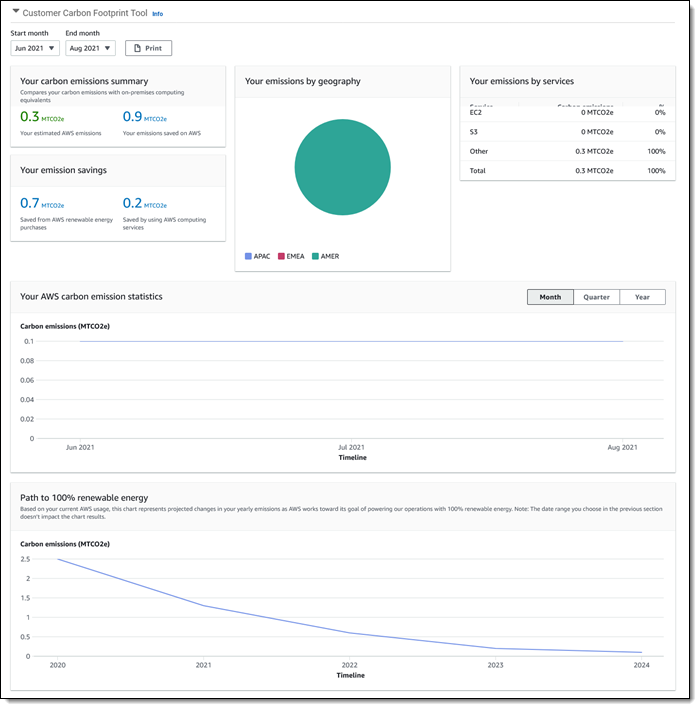
\includegraphics[width=0.8\textwidth]{imagenes/AWS_1.png}
  \captionof{figure}{Vista de la herramienta AWS Customer Carbon Footprint Tool.}
\end{center}
\subsection*{Puntos fuertes:}
\begin{itemize}
  \item \textbf{Cobertura histórica}: muestra datos desde enero de 2020, con hasta 36 meses de historial disponible.
  \item \textbf{Estándares reconocidos}: se basa en el \textbf{GHG Protocol} y cuenta con verificación independiente según \textbf{ISO 14064}\footnote{Norma internacional para cuantificar y reportar emisiones de gases de efecto invernadero; asegura buen uso de metodologías.}.
  \item \textbf{Detalle granular}: permite analizar emisiones por servicio y región, facilitando la toma de decisiones.
  \item \textbf{Cálculo de ahorros}: estima reducciones de emisiones gracias al uso de energía renovable, comparando métodos \textit{location-based} vs. \textit{market-based}.
  \item \textbf{Exportación de datos}: facilita la integración con otras herramientas de análisis y generación de informes mediante \textbf{Data Exports}.
  \item \textbf{Consolidación de cuentas}: permite visualizar métricas de múltiples cuentas dentro de una organización usando \textbf{AWS Organizations}.
\end{itemize}
\subsection*{Puntos débiles:}
\begin{itemize}
  \item \textbf{No incluye Scope 3}: no abarca emisiones indirectas de la cadena de valor, como la fabricación del hardware; se espera en futuras versiones.
  \item \textbf{Retraso en los datos}: las métricas tienen un desfase de tres meses, lo que impide análisis en tiempo real.
  \item \textbf{Acceso restringido}: requiere permisos \textbf{IAM}\footnote{Sistema de control de acceso de AWS: defines quién puede ver o exportar datos de emisiones de carbono en tu cuenta.} específicos para consultar la herramienta.
  \item \textbf{Ecosistema cerrado}: está limitado al entorno AWS, sin integración multicloud ni comparativa con infraestructura local (\textit{on-premises})\footnote{Infraestructura propia (servidores físicos) cuya huella de carbono mides por tu cuenta, fuera de la nube de AWS.}.
  \item \textbf{Sin visión futura}: no proyecta emisiones futuras del cliente ni las compara con la hoja de ruta renovable de AWS.
\end{itemize}

\section*{Impact Framework}

\href{https://greensoftware.foundation/}{https://greensoftware.foundation/}

\href{https://if.greensoftware.foundation/}{https://if.greensoftware.foundation/}

\href{https://if.greensoftware.foundation/intro}{https://if.greensoftware.foundation/intro}

Impact Framework es un conjunto de herramientas diseñado para medir las
emisiones de carbono generadas por el uso del software. Se basa en una
arquitectura modular, es decir, está compuesto por partes independientes
llamadas \textbf{plugins}\footnote{es un componente de software que añade una funcionalidad específica a un programa principal. Se utiliza para extender las capacidades de una aplicación sin modificar su núcleo} que se pueden combinar según las necesidades del análisis. Su
objetivo es transformar métricas observables como el uso de CPU, los
\textbf{bytes transferidos}\footnote{Cantidad de datos enviados o recibidos;
  base para estimar la energía consumida por la red y emisiones.} o el número de
visitas a páginas en estimaciones del impacto ambiental, es decir, cuántas
emisiones de CO\textsubscript{2} se producen.

Existen dos tipos principales de plugins:

\begin{itemize}
  \item \textbf{Plugins de observación}: recogen datos del sistema. Por ejemplo, el plugin \texttt{webpage-impact} mide cuántos \textbf{bytes transferidos} al cargar una página web.
  \item \textbf{Plugins de cálculo}: transforman esos datos en estimaciones de emisiones. Un ejemplo es el plugin \texttt{co2js}, que utiliza modelos como \textbf{Sustainable Web Design}\footnote{Modelo que asigna emisiones de CO\textsubscript{2} según el tamaño y transferencia de recursos de una página web.} u \textbf{OneByte}\footnote{Modelo que calcula emisiones de carbono por byte transferido, basado en estadísticas de consumo energético.} para calcular el carbono emitido a partir de los \textbf{bytes transferidos}. Estos modelos asumen valores promedio de consumo energético por cada byte enviado o recurso digital utilizado.
\end{itemize}

Se puede aplicar a varios escenarios relacionados con el desarrollo de
software. Por ejemplo, permite evaluar el impacto ambiental de sitios web
midiendo las emisiones por carga de página según los \textbf{bytes
  transferidos}. También se puede usar
para analizar el consumo de red y CPU en \textbf{APIs}\footnote{Conjunto de
  reglas que permite la comunicación entre aplicaciones; su uso implica
  transferencia de datos.} o \textbf{microservicios}\footnote{Componente de
  software independiente que realiza una función específica; su rendimiento
  afecta emisiones.}, e integrarse en procesos de desarrollo automatizados
(\textbf{pipelines CI/CD}\footnote{Secuencia automatizada de integración,
  pruebas y despliegue de software; ideal para medir emisiones por versión.})
para comprobar que nuevas versiones del software no incrementen su huella de
carbono. Además, sirve para comparar alternativas tecnológicas desde un enfoque
de sostenibilidad.

Se puede probar instalándolo en nuestro equipo mediante el \textbf{gestor de
  paquetes} npm\footnote{Herramienta que instala y gestiona librerías o
  herramientas, como npm para proyectos JavaScript.}:

\begin{tcolorbox}[colback=codebackground, colframe=codeborder, boxrule=0.8pt, arc=0mm, boxsep=5pt, left=5pt, right=5pt, top=5pt, bottom=5pt]
  \begin{lstlisting}[language=bash]
  npm install -g @grnsft/if
  \end{lstlisting}
\end{tcolorbox}

Creamos un fichero \textbf{IMP}\footnote{Archivo de configuración de Impact
  Framework en formato YAML; define qué métricas y plugins usar.} con la
extensión \textbf{.yml}\footnote{Archivo de configuración de Impact Framework
  en formato YAML; define qué métricas y plugins usar.}, el cual contendrá las
configuraciones y los datos necesarios para medir el impacto energético y
ambiental de nuestra aplicación:

\begin{center}
  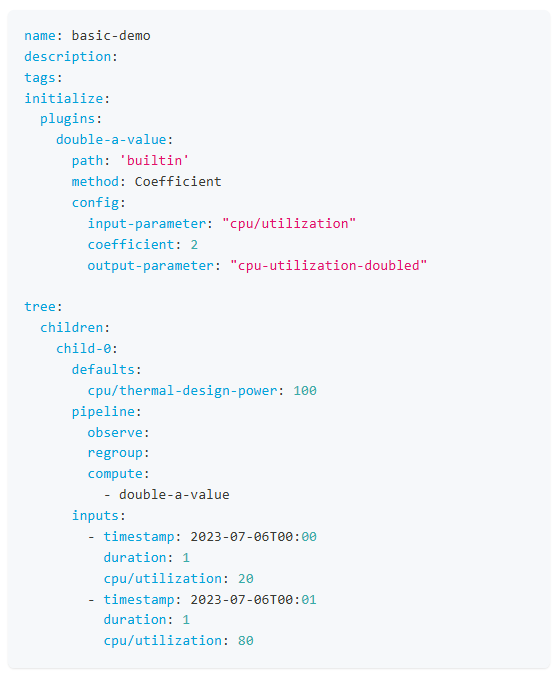
\includegraphics[width=0.8\textwidth]{imagenes/IF_1.png}
  \captionof{figure}{Archivo IMP de ejemplo}
\end{center}

Tras esto, lo podemos ejecutar con:

\begin{tcolorbox}[colback=codebackground, colframe=codeborder, boxrule=0.8pt, arc=0mm, boxsep=5pt, left=5pt, right=5pt, top=5pt, bottom=5pt]
  \begin{lstlisting}[language=bash]
  if-run --IMP <path-to-your-IMP>
  \end{lstlisting}
\end{tcolorbox}

\subsection*{Puntos fuertes:}

\begin{itemize}
  \item \textbf{Arquitectura modular}: al estar basado en plugins, se puede personalizar y extender fácilmente según el software que se quiera analizar.
  \item \textbf{Flexibilidad}: sirve para diferentes tipos de software, como páginas web, apps móviles o sistemas en la \textbf{nube}.
  \item \textbf{Modelos validados}: usa modelos conocidos como \textbf{Sustainable Web Design} y \textbf{OneByte} para realizar las estimaciones de carbono, lo que le da credibilidad.
  \item \textbf{Código abierto}: cualquier persona puede usarlo y mejorarlo, ya que es libre y está apoyado por la Green Software Foundation.
  \item \textbf{Enfoque automatizable}: permite integrarse en procesos automáticos de desarrollo, usando un archivo de configuración en formato \textbf{YAML}\footnote{Formato de texto legible para definir configuraciones, como parámetros de cálculo de emisiones.}.
\end{itemize}

\subsection*{Puntos débiles:}

\begin{itemize}
  \item \textbf{Precisión limitada}: como se basa en estimaciones, los resultados dependen de suposiciones generales que no siempre se ajustan a cada caso concreto. \href{https://www.npmjs.com/package/@tgwf/co2}{https://www.npmjs.com/package/@tgwf/co2}
  \item \textbf{Curva de aprendizaje}: es necesario tener conocimientos técnicos para configurarlo correctamente, especialmente el archivo \textbf{IMP} y la selección de plugins.
  \item \textbf{Cobertura parcial}: es una herramienta relativamente nueva y todavía tiene pocos plugins disponibles, lo que limita su alcance actual.
\end{itemize}

\subsection*{Carbon Aware SDK}

\href{https://greensoftware.foundation/}{https://greensoftware.foundation/}

\href{https://carbon-aware-sdk.greensoftware.foundation/}{https://carbon-aware-sdk.greensoftware.foundation/}

\href{https://carbon-aware-sdk.greensoftware.foundation/docs/overview}{https://carbon-aware-sdk.greensoftware.foundation/docs/overview}

Carbon Aware SDK es un conjunto de herramientas diseñado para ayudar a las
aplicaciones a adaptar su comportamiento en función de la \textbf{intensidad de
  carbono}\footnote{Gramos de CO\textsubscript{2} emitidos por cada kWh
  producido; indica cuán limpia o sucia es la energía consumida.} de la red
eléctrica, considerando el momento y la ubicación geográfica. Su objetivo es
permitir decisiones sostenibles en tiempo real, optimizando tareas para
ejecutarse cuando hay mayor disponibilidad de energía limpia.

La herramienta incluye tanto una \textbf{API web} como una \textbf{interfaz de línea de comandos
  (CLI)}\footnote{Interfaz de línea de comandos; herramienta basada en texto para
  ejecutar funciones directamente.}, ofreciendo flexibilidad para distintos
\textbf{entornos de despliegue}\footnote{Conjunto de infraestructuras y
  configuraciones donde corre el software (on‑premises, nube, contenedores).}. La
\textbf{API web} está orientada a
\textbf{implementaciones centralizadas y auditables}\footnote{Despliegues
  controlados desde un único punto con trazabilidad completa de quién hizo qué y
  cuándo.}, mientras que la \textbf{CLI} resulta útil
en \textbf{sistemas heredados}\footnote{Aplicaciones o infraestructuras
  antiguas que aún están en producción y pueden no soportar nuevas
  integraciones.} o \textbf{pipelines CI/CD}, garantizando una funcionalidad coherente en ambos casos.

Carbon Aware SDK se basa en una arquitectura de
\textbf{plugins} que permite integrar múltiples fuentes
de datos externas, como \textbf{WattTime}\footnote{Proveedor de datos en tiempo
  real y previsiones de intensidad de carbono de redes eléctricas.} o
\textbf{Electricity Maps}\footnote{Plataforma que ofrece datos históricos, en
  tiempo real y pronósticos de mezcla energética y emisiones.}, y estandariza
automáticamente las unidades de medida a
\textbf{gCO\textsubscript{2}/kWh}\footnote{Unidad de medida que expresa gramos
  de CO\textsubscript{2} emitidos por cada kilovatio-hora consumido.}. También es
capaz de agregar datos por región, ofreciendo una visión más completa del
impacto energético.

Está pensado para ser usado en aplicaciones que pueden modificar su
comportamiento: por ejemplo, diferir tareas intensivas en momentos de menor
huella de carbono o adaptarse en \textbf{entornos distribuidos y
  multinube}\footnote{Infraestructuras repartidas en varias regiones o
  proveedores de nube, cada una con distinta intensidad de carbono.} que
requieren ajustarse a diferentes niveles de intensidad energética según la
localización.

Para usarlo por \textbf{CLI} necesitamos
tener \textbf{.NET Core}\footnote{Plataforma de ejecución multiplataforma de
  Microsoft para construir y ejecutar aplicaciones.} (o usar
\textbf{Docker}\footnote{Motor de contenedores que empaqueta aplicaciones con
  sus dependencias para ejecución aislada.} con VSCode y Remote Containers).
Clonamos el repositorio con:

\begin{tcolorbox}[colback=codebackground, colframe=codeborder, boxrule=0.8pt, arc=0mm, boxsep=5pt, left=5pt, right=5pt, top=5pt, bottom=5pt]
  \begin{lstlisting}[language=bash]
git clone https://github.com/Green-Software-Foundation/carbon-aware-sdk.git
\end{lstlisting}
\end{tcolorbox}

y accedemos a la carpeta:

\begin{tcolorbox}[colback=codebackground, colframe=codeborder, boxrule=0.8pt, arc=0mm, boxsep=5pt, left=5pt, right=5pt, top=5pt, bottom=5pt]
  \begin{lstlisting}[language=bash]
cd carbon-aware-sdk/src/CarbonAware.CLI/src
\end{lstlisting}
\end{tcolorbox}

Podemos usar datos simulados por defecto o configurar variables de entorno si
tenemos cuenta en \textbf{WattTime} o
\textbf{Electricity Maps}. Ejecutamos
comandos con:

\begin{tcolorbox}[colback=codebackground, colframe=codeborder, boxrule=0.8pt, arc=0mm, boxsep=5pt, left=5pt, right=5pt, top=5pt, bottom=5pt]
  \begin{lstlisting}[language=bash]
dotnet run
\end{lstlisting}
\end{tcolorbox}

Por ejemplo, para obtener emisiones de dos regiones en un período de tiempo:

\begin{tcolorbox}[colback=codebackground, colframe=codeborder, boxrule=0.8pt, arc=0mm, boxsep=5pt, left=5pt, right=5pt, top=5pt, bottom=5pt]
  \begin{lstlisting}[language=bash]
dotnet run emissions -l eastus,uksouth -s 2022-08-23T11:15 -e 2022-08-23T11:20
\end{lstlisting}
\end{tcolorbox}

\begin{center}
  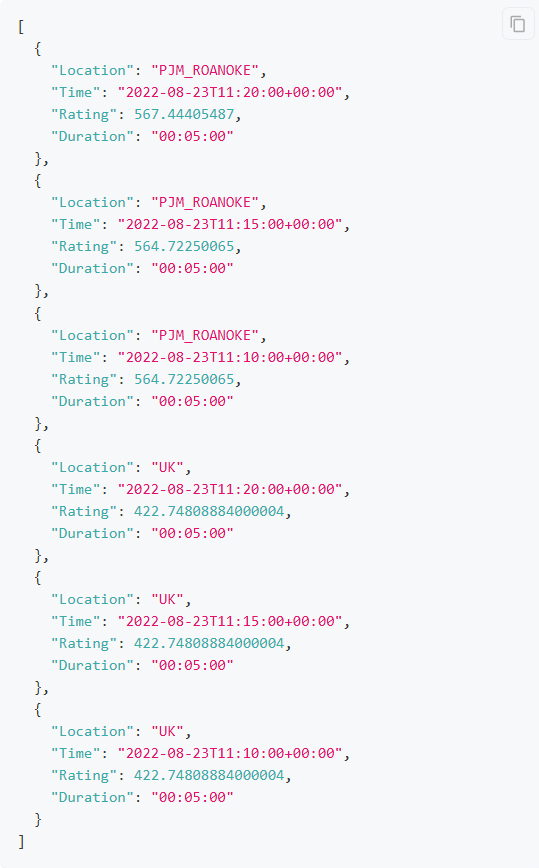
\includegraphics[width=0.8\textwidth]{imagenes/CASDK_1.png}
  \captionof{figure}{Salida del comando de emisiones para dos regiones.}
\end{center}

Y para obtener el mejor momento y la región con menos emisiones en una ventana
temporal específica:

\begin{tcolorbox}[colback=codebackground, colframe=codeborder, boxrule=0.8pt, arc=0mm, boxsep=5pt, left=5pt, right=5pt, top=5pt, bottom=5pt]
  \begin{lstlisting}[language=bash]
dotnet run emissions -l eastus,uksouth -s 2022-08-23T00:00 -e 2022-08-23T23:59 --best
\end{lstlisting}
\end{tcolorbox}

\begin{center}
  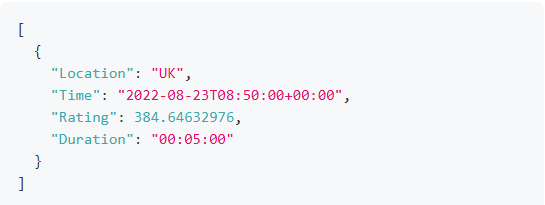
\includegraphics[width=0.8\textwidth]{imagenes/CASDK_2.png}
  \captionof{figure}{Salida del comando para encontrar el mejor momento y región para minimizar emisiones.}
\end{center}

Si preferimos la \textbf{API web} en
lugar de la \textbf{CLI}, podemos ejecutarla y
acceder a \href{http://localhost:5073}{http://localhost:5073/} y hacer llamadas
desde la consola:

\begin{tcolorbox}[colback=codebackground, colframe=codeborder, boxrule=0.8pt, arc=0mm, boxsep=5pt, left=5pt, right=5pt, top=5pt, bottom=5pt]
  \begin{lstlisting}[language=bash]
curl http://localhost:5073/locations
\end{lstlisting}
\end{tcolorbox}

Esto devolverá un \textbf{JSON}\footnote{Formato de intercambio de datos basado
  en texto, común en respuestas de APIs.} con todas las ubicaciones disponibles.
También es posible generar clientes en más de 50 lenguajes distintos usando
\textbf{OpenAPI Generator}\footnote{Herramienta que genera clientes y
  servidores en varios lenguajes a partir de especificaciones OpenAPI.}, lo que
facilita la integración en cualquier \textbf{stack}\footnote{Conjunto de
  tecnologías (lenguajes, frameworks, bases de datos) utilizadas conjuntamente en
  un proyecto.}.

\subsection*{Puntos fuertes:}

\begin{itemize}
  \item \textbf{Optimización dinámica}: ajusta la ejecución del software según la disponibilidad de energía limpia.
  \item \textbf{Versatilidad de uso}: ofrece tanto \textbf{API web} como \textbf{CLI}, adaptándose a distintos entornos de desarrollo.
  \item \textbf{Integración con proveedores diversos}: conecta con servicios como \textbf{WattTime} o \textbf{Electricity Maps} mediante \textbf{plugins}.
  \item \textbf{Estandarización automática}: convierte unidades dispares a \textbf{gCO\textsubscript{2}/kWh} para facilitar el análisis.
  \item \textbf{Agregación regional}: combina datos de múltiples fuentes según la ubicación geográfica.
\end{itemize}

\subsection*{Puntos débiles:}

\begin{itemize}
  \item \textbf{Requiere implementación}: es necesario modificar el código de la aplicación para aprovechar sus funcionalidades.
  \item \textbf{Dependencia de terceros}: la precisión depende de la calidad de los datos de \textbf{WattTime} o \textbf{Electricity Maps}.
  \item \textbf{Curva de aprendizaje}: integrar la herramienta correctamente puede requerir esfuerzo técnico para configurar \textbf{.NET Core}, \textbf{Docker} y \textbf{pipelines CI/CD}.
  \item \textbf{Información limitada}: no ofrece desglose de la \textbf{mezcla energética}\footnote{Composición porcentual de fuentes renovables y no renovables que alimentan una red eléctrica.}, solo la \textbf{intensidad agregada de carbono}\footnote{Valor promedio de intensidad de carbono calculado a partir de múltiples fuentes o regiones.}.
  \item \textbf{Conectividad constante}: necesita acceso continuo a las APIs, lo que lo hace inviable en entornos con mala conexión.
\end{itemize}

\section*{Cloud Carbon Footprint}

\href{https://www.cloudcarbonfootprint.org/}{https://www.cloudcarbonfootprint.org/}

\href{https://www.cloudcarbonfootprint.org/docs/}{https://www.cloudcarbonfootprint.org/docs/}

Cloud Carbon Footprint es una herramienta gratuita y de código abierto diseñada
para visualizar el impacto ambiental de las infraestructuras cloud\footnote{Conjunto de recursos tecnol´ogicos (como servidores, redes y almacenamiento) ofrecidos por provee-
dores en la nube para ejecutar servicios y aplicaciones.} de
proveedores como \textbf{AWS}, \textbf{Azure}\footnote{Plataforma de
  servicios en la nube proporcionada por Microsoft, similar a AWS y GCP.} y
\textbf{GCP}\footnote{Google Cloud Platform, conjunto de servicios de
  computación en la nube desarrollados por Google.}. Analiza los datos de
facturación y uso para estimar el consumo energético y las emisiones asociadas.
Su objetivo es proporcionar a las empresas una visión detallada de su huella de
carbono en la nube, ayudándolas a tomar decisiones informadas para optimizar
recursos y reducir emisiones.

La herramienta es \textbf{multicloud}\footnote{Estrategia o herramienta que
  permite trabajar simultáneamente con múltiples proveedores de servicios
  cloud.}, lo que significa que es compatible con AWS, Azure y GCP, y permite
desglosar las métricas por cuenta, servicio y periodo. Cloud Carbon Footprint
también ofrece recomendaciones específicas para la optimización de costos y la
reducción de emisiones, tales como \textit{rightsizing}\footnote{Técnica de
  optimización que consiste en ajustar los recursos cloud al tamaño y uso
  necesario, evitando sobredimensionamiento.} o eliminación de \textbf{instancias
  inactivas}\footnote{Máquina virtual u otro recurso en la nube que está
  encendido pero no está siendo utilizado, consumiendo energía y generando costes
  innecesarios.}. Además, cuenta con una buena variedad de opciones de
visualización, como paneles interactivos y la capacidad de exportar datos en
formatos \textbf{CSV} y \textbf{JSON}.

Una de las funcionalidades destacadas es la estimación de ahorros de costo y
carbono a futuro, proporcionando proyecciones basadas en las recomendaciones
aplicadas. Esto permite a las organizaciones priorizar sus acciones de
optimización y tomar medidas para reducir tanto los costos como el impacto
ambiental de sus \textbf{infraestructuras cloud}.

Para comenzar con Cloud Carbon Footprint, la forma más recomendada es crear una
aplicación independiente usando la línea de comandos. Esto se hace con el
paquete ejecutando el comando del gestor de paquetes npx:

\begin{tcolorbox}[colback=codebackground, colframe=codeborder, boxrule=0.8pt, arc=0mm, boxsep=5pt, left=5pt, right=5pt, top=5pt, bottom=5pt]
  \begin{lstlisting}[language=bash]
  npx @cloud-carbon-footprint/create-app
  \end{lstlisting}
\end{tcolorbox}

lo que te permite configurar rápidamente una instancia funcional de la
aplicación con mínima personalización.

Terminamos de configurarlo con nuestras cuentas de los distintos servicios que
queremos analizar con:

\begin{tcolorbox}[colback=codebackground, colframe=codeborder, boxrule=0.8pt, arc=0mm, boxsep=5pt, left=5pt, right=5pt, top=5pt, bottom=5pt]
  \begin{lstlisting}[language=bash]
  cd my-ccf-app
  yarn guided-install
  \end{lstlisting}
\end{tcolorbox}

Inicializamos la aplicación que hemos creado con:

\begin{tcolorbox}[colback=codebackground, colframe=codeborder, boxrule=0.8pt, arc=0mm, boxsep=5pt, left=5pt, right=5pt, top=5pt, bottom=5pt]
  \begin{lstlisting}[language=bash]
  yarn start
  \end{lstlisting}
\end{tcolorbox}

Lo cual nos sirve el frontend en
\href{http://localhost:3000}{http://localhost:3000}, en el cual se nos muestra
toda la información y podemos decidir los filtros y opciones que queramos para
una mejor visualización:

\begin{center}
  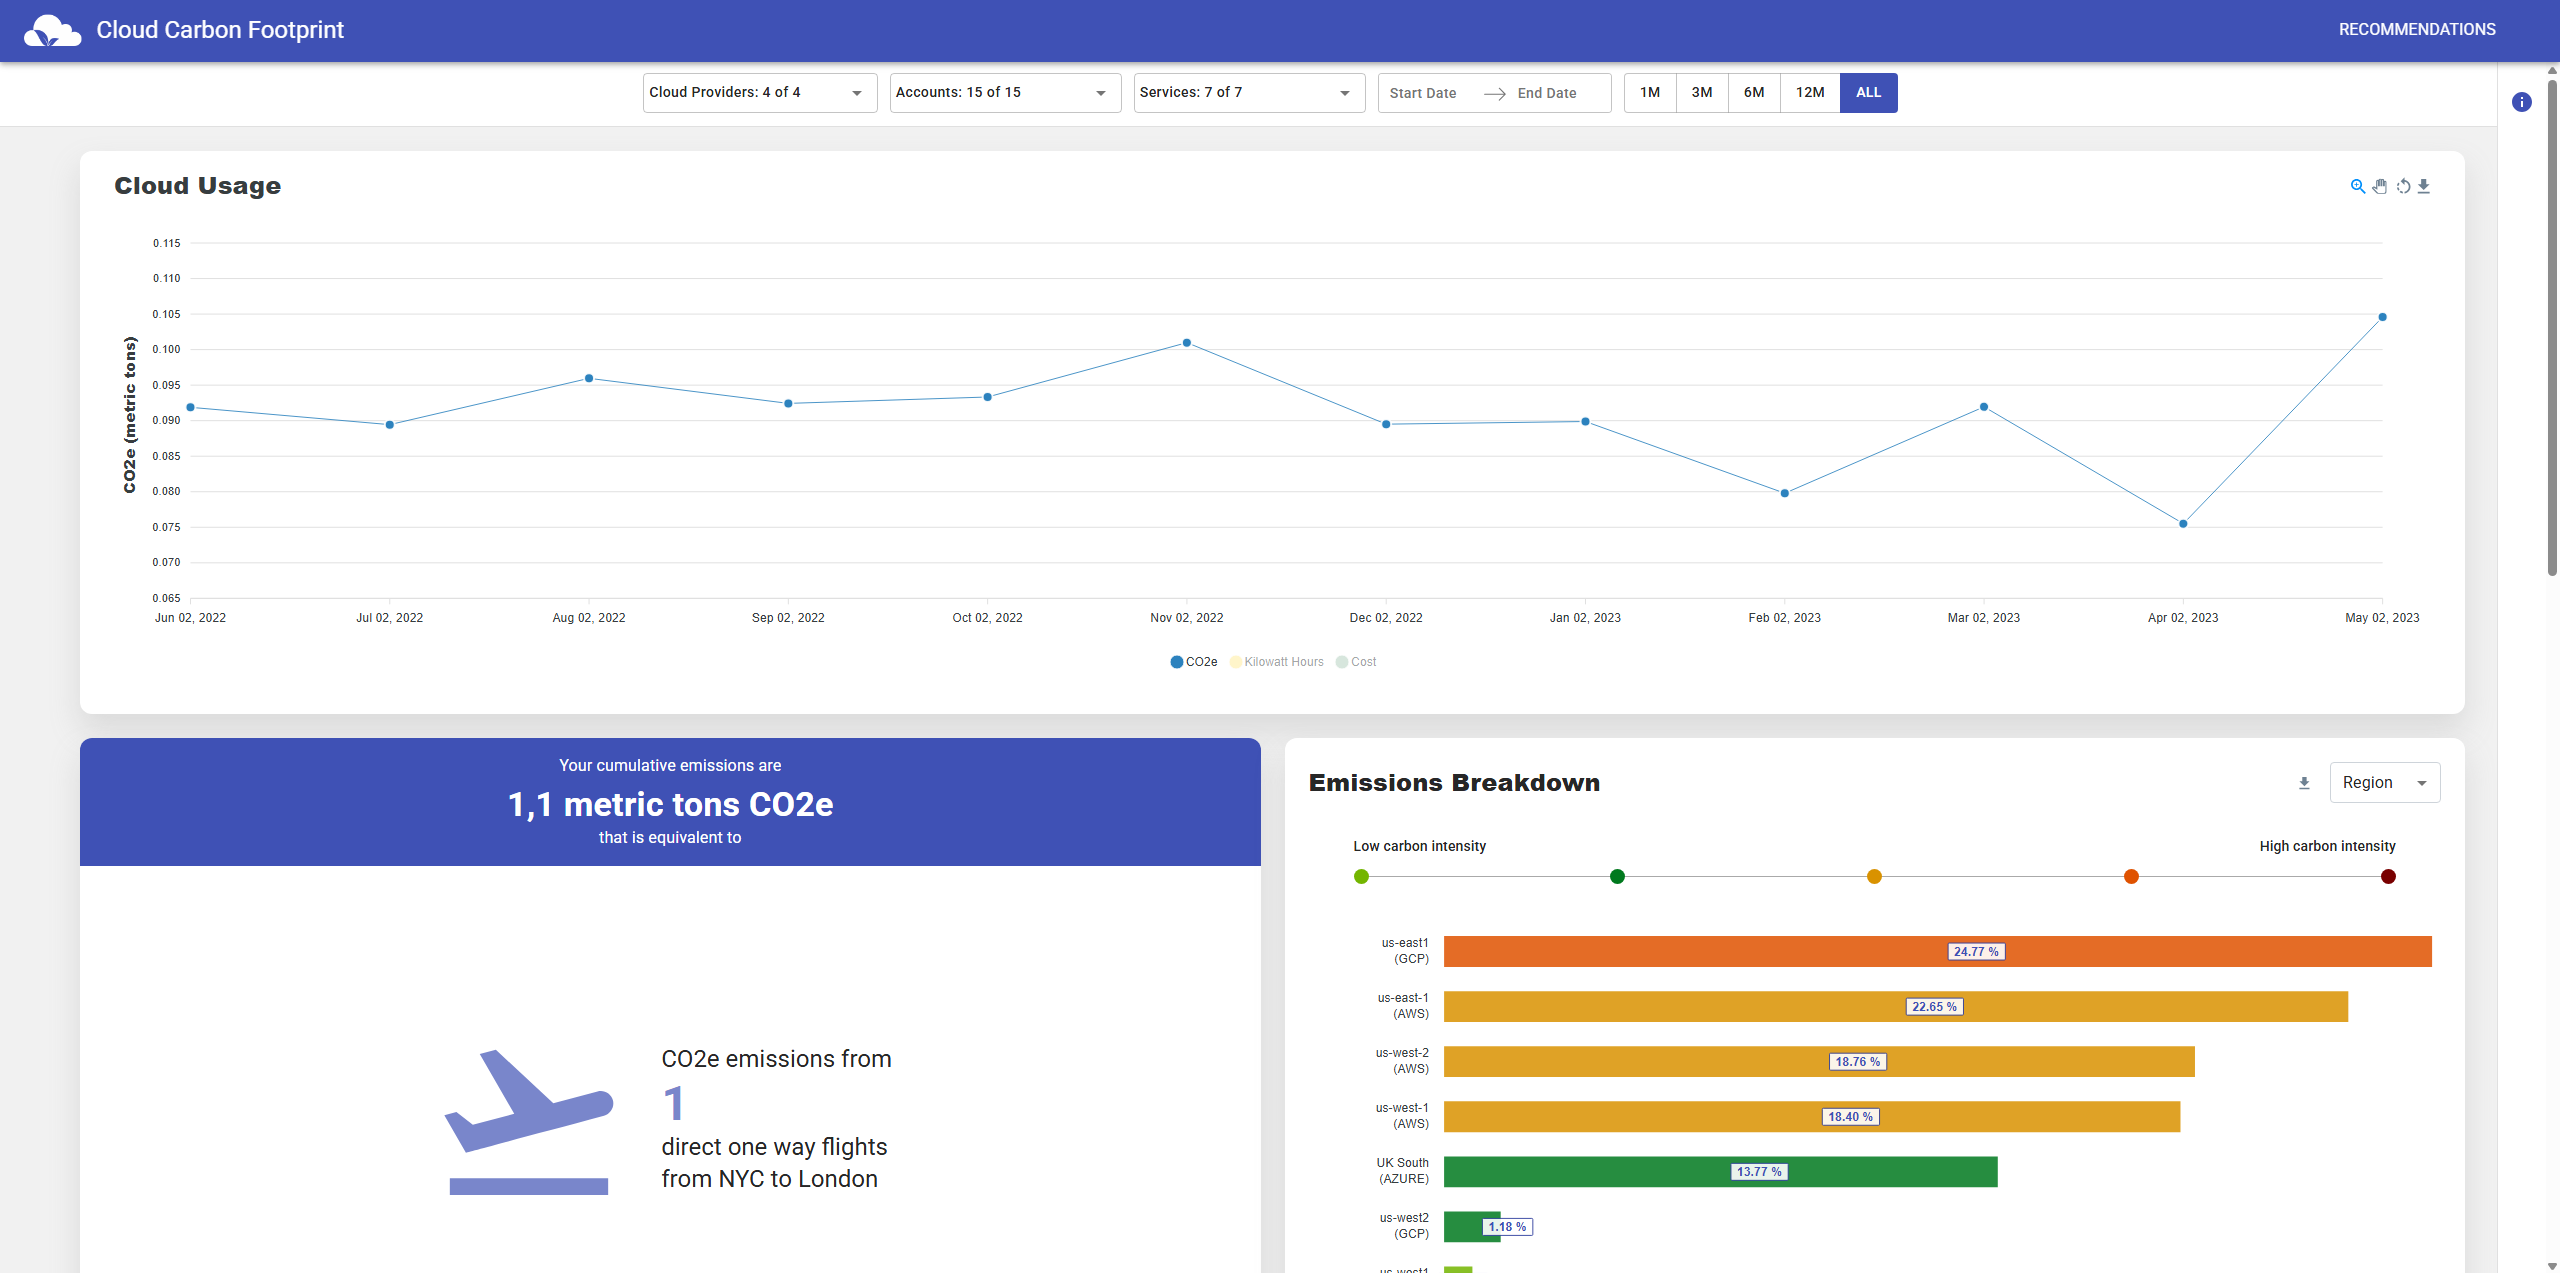
\includegraphics[width=0.8\textwidth]{imagenes/CCF_1.png}
  \captionof{figure}{Panel principal de Cloud Carbon Footprint}
\end{center}

\begin{center}
  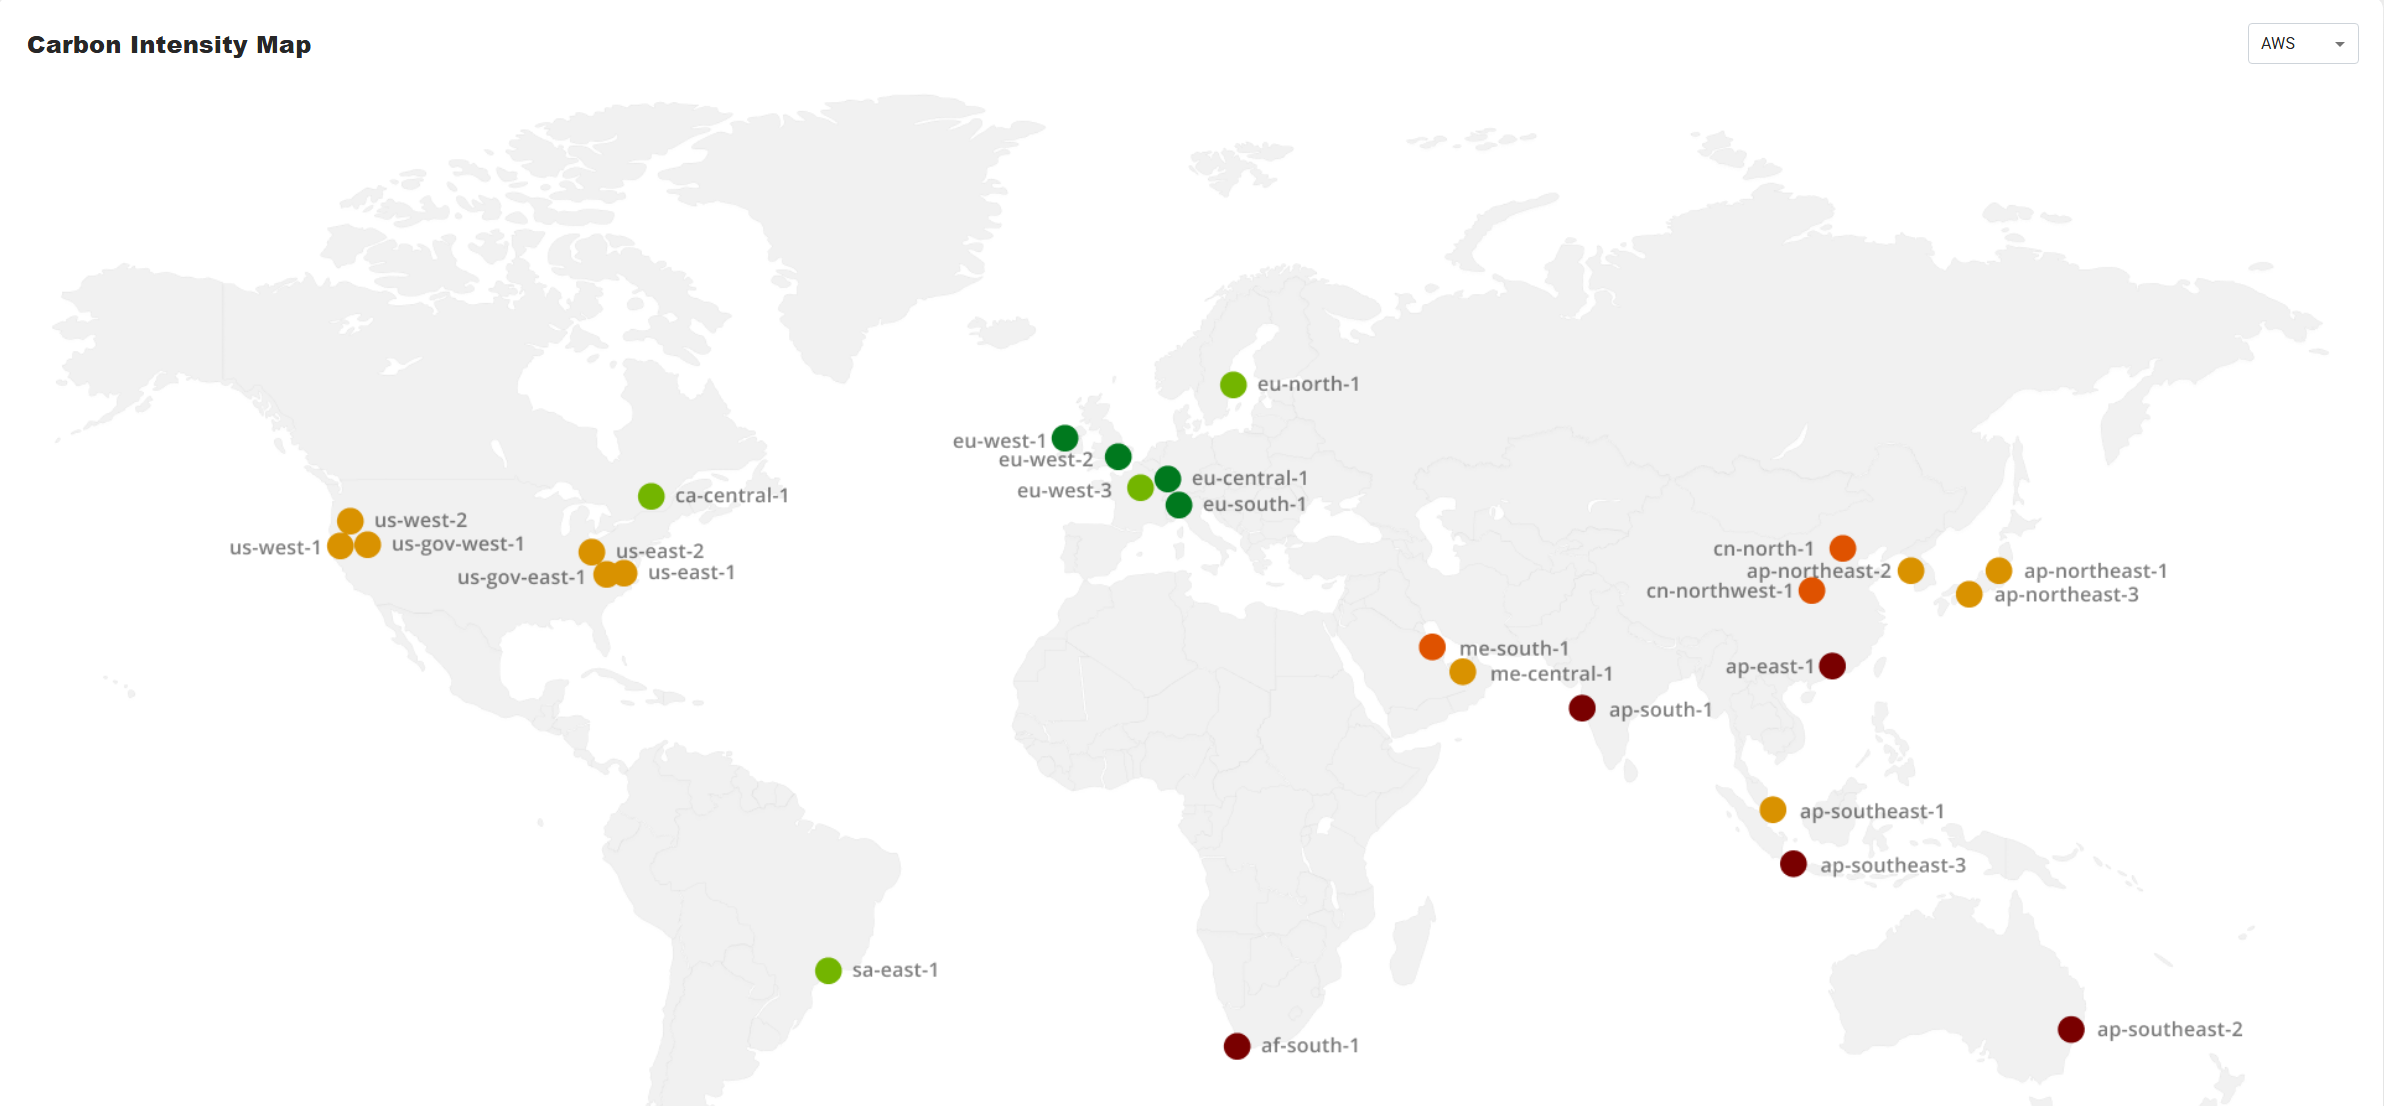
\includegraphics[width=0.8\textwidth]{imagenes/CCF_2.png}
  \captionof{figure}{Visualización de métricas en Cloud Carbon Footprint}
\end{center}

También puedes clonar el repositorio y configurar la aplicación localmente para
realizar los cambios que necesites. Otra opción es ejecutar la aplicación en un
\textbf{entorno efímero}\footnote{Entorno temporal de desarrollo o ejecución
  que se puede eliminar fácilmente tras su uso, sin dejar persistencia local.}
usando \textbf{Gitpod}\footnote{Plataforma basada en la nube que permite lanzar
  entornos de desarrollo preconfigurados directamente desde un navegador.}, lo
que te permite probar la aplicación sin configuraciones locales, aunque es
menos flexible para personalización a largo plazo.

\subsection*{Puntos fuertes:}

\begin{itemize}
  \item \textbf{Compatibilidad multicloud}: integración con los principales proveedores de nube (AWS, Azure y GCP).
  \item \textbf{Análisis detallado}: desglose de emisiones por cuenta, servicio y período, facilitando la identificación de áreas problemáticas.
  \item \textbf{Recomendaciones accionables}: sugiere optimizaciones específicas con estimaciones de ahorro en costos y emisiones.
  \item \textbf{Visualización interactiva}: paneles personalizables que facilitan la comprensión de datos complejos.
  \item \textbf{Código abierto}: permite personalización y contribuciones de la comunidad.
\end{itemize}

\subsection*{Puntos débiles:}

\begin{itemize}
  \item \textbf{Configuración inicial}: requiere conocimientos técnicos para la configuración de proveedores cloud.
  \item \textbf{Precisión variable}: las estimaciones pueden variar según la calidad y completitud de los datos de facturación disponibles.
  \item \textbf{Dependencia de datos externos}: requiere acceso a las APIs o datos de facturación de los proveedores cloud.
\end{itemize}

\section*{Carbonalyser}

\href{https://theshiftproject.org/en/}{https://theshiftproject.org/en/}

\href{https://addons.mozilla.org/es-ES/firefox/addon/carbonalyser/}{https://addons.mozilla.org/es-ES/firefox/addon/carbonalyser/}

\href{https://github.com/carbonalyser/Carbonalyser}{https://github.com/carbonalyser/Carbonalyser}

\textbf{Carbonalyser} es una extensión de navegador gratuita que permite visualizar el impacto ambiental del uso de Internet. Estima las emisiones de carbono derivadas de la navegación web a partir de la cantidad de datos transmitidos, utilizando el modelo \textbf{"1byte"}\footnote{Modelo de estimación del consumo energético y emisiones de CO\textsubscript{2} basado en la cantidad de datos transmitidos por Internet, propuesto por \textit{The Shift Project}.} desarrollado por \textit{The Shift Project}. A través de esta herramienta, los usuarios pueden comprender mejor el impacto de su navegación en términos de consumo energético y emisiones de CO\textsubscript{2}, ajustado a la intensidad de carbono de su región.

Está disponible para \textbf{Firefox}, y existen versiones \textit{fork} para
\textbf{Chrome} y \textbf{Edge}, lo que facilita su instalación y uso. La
extensión procesa toda la información de manera \textbf{local}, sin enviar
datos a servidores externos, lo que garantiza la privacidad del usuario. La
visualización es intuitiva, mostrando un ranking de sitios web, datos
transmitidos y comparaciones con actividades físicas cotidianas (como el uso de
un móvil o la conducción).

Carbonalyser es además código abierto bajo licencia MIT, con el código alojado
en \textbf{GitHub}\footnote{Plataforma de desarrollo colaborativo basada en Git que permite almacenar, compartir y revisar
código fuente.}. Permite configurar la ubicación eléctrica para ajustar las
estimaciones a la \textbf{intensidad de carbono regional}\footnote{Valor medio de emisiones por kWh en una región concreta, utilizado para estimar el impacto energético del centro de datos.}, ayudando a que el análisis
sea más contextual y educativo.

Al ser una extensión del navegador, es tan fácil como obtenerla como cualquier
otra mediante el buscador de extensiones del navegador.

\begin{center}
  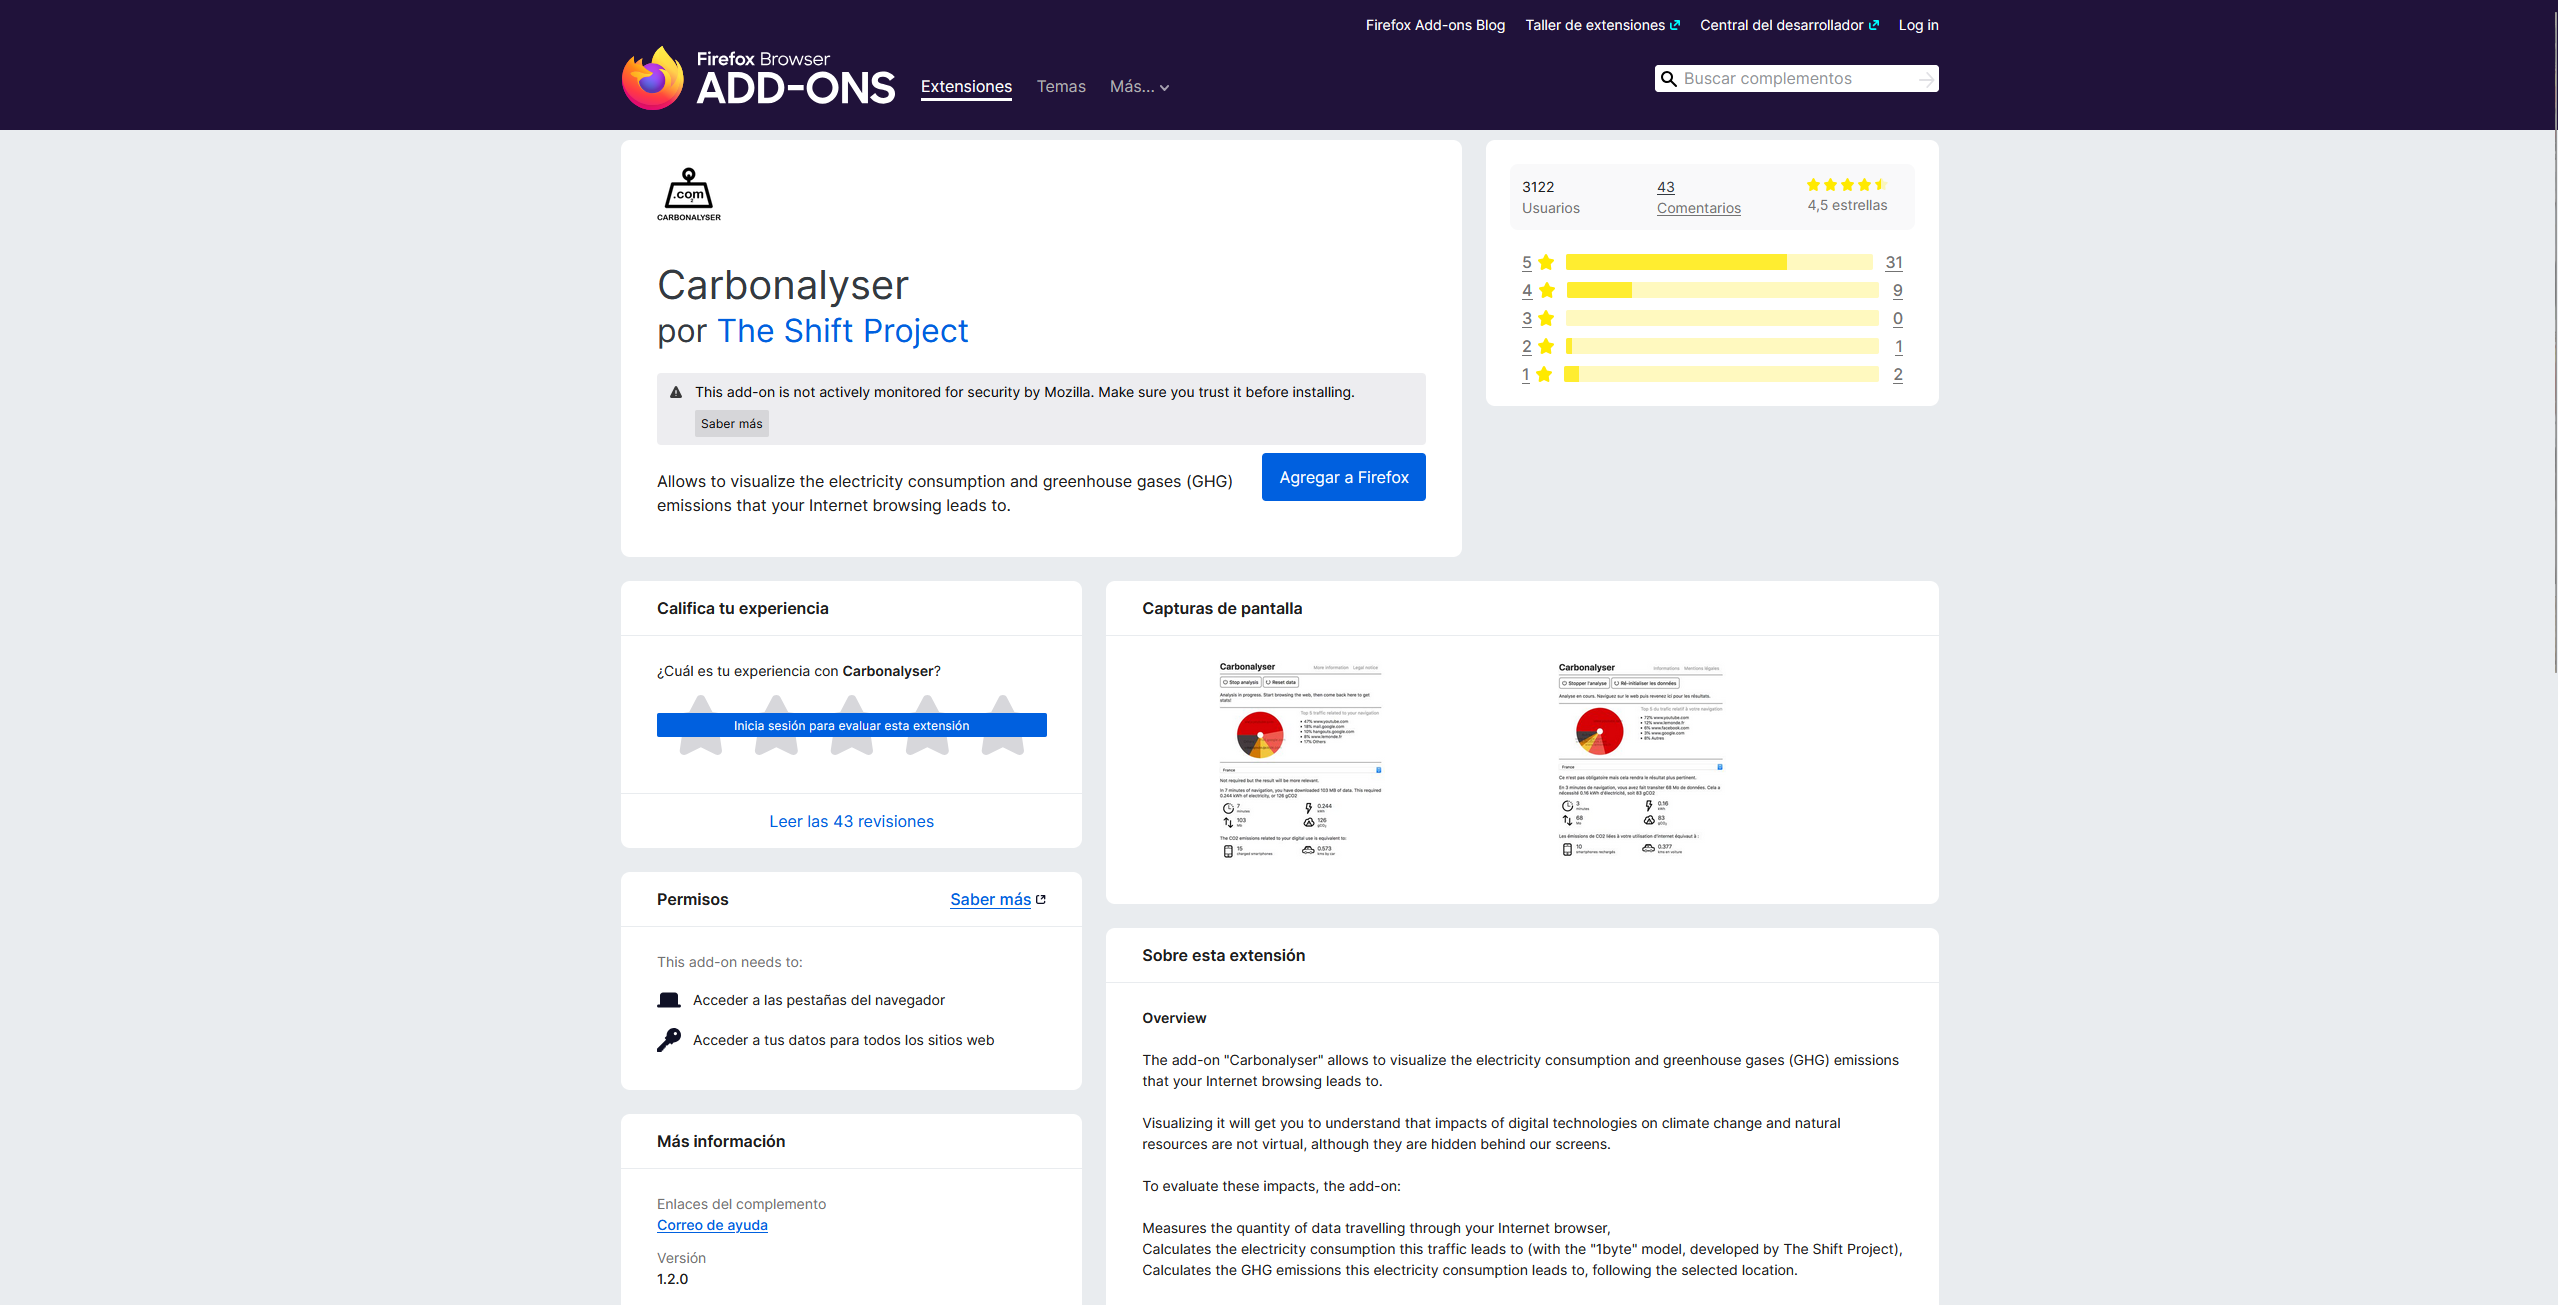
\includegraphics[width=0.8\textwidth]{imagenes/Carbonalyser_1.png}
  \captionof{figure}{Instalación de Carbonalyser en Firefox}
\end{center}

Una vez instalada podremos iniciar un análisis que analizará nuestra actividad
en el navegador a partir de ese punto.

\begin{center}
  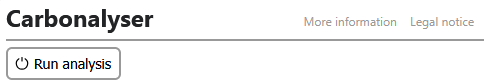
\includegraphics[width=0.8\textwidth]{imagenes/Carbonalyser_2.png}
  \captionof{figure}{Interfaz de monitorización de Carbonalyser}
\end{center}

Una vez hemos terminado, volvemos e indicamos nuestra región y con esto nos
dirá toda la información relevante en relación al análisis.

\begin{center}
  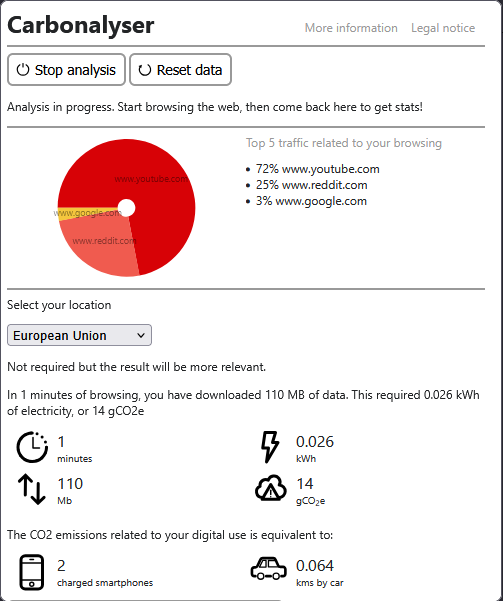
\includegraphics[width=0.8\textwidth]{imagenes/Carbonalyser_3.png}
  \captionof{figure}{Resultados del análisis de emisiones}
\end{center}

\subsection*{Puntos fuertes:}

\begin{itemize}
  \item \textbf{Muy fácil de usar}: instalación rápida en Firefox (y forks disponibles para Chrome y Edge).
  \item \textbf{Procesamiento 100\% local}: no transmite datos a terceros, garantizando privacidad.
  \item \textbf{Visualización clara y educativa}: rankings, comparativas y equivalencias comprensibles.
  \item \textbf{Código abierto y gratuito}: bajo licencia MIT, con comunidad en GitHub.
  \item \textbf{Cálculo adaptado por región}: permite configurar la localización eléctrica del usuario.
  \item \textbf{Herramienta útil para educación}: ideal para concienciar sobre sostenibilidad digital.
\end{itemize}

\subsection*{Puntos débiles:}

\begin{itemize}
  \item \textbf{Limitado al tráfico web}: no mide el impacto de componentes fuera del navegador.
  \item \textbf{Basado en modelos generalistas}: utiliza estimaciones teóricas ("1byte"), no mediciones de hardware reales.
  \item \textbf{No almacena datos históricos}: se reinicia al cerrar el navegador, sin seguimiento continuo.
  \item \textbf{No integrable en otros sistemas}: no puede incorporarse a software externo o pipelines.
  \item \textbf{Desarrollo inactivo}: última versión publicada en 2020, con escasa evolución desde entonces.
  \item \textbf{Permisos elevados}: requiere acceso a pestañas y solicitudes web, lo que puede generar reticencias en entornos corporativos.
  \item \textbf{Cálculo adaptado por región limitado}: Solo permite elegir entre regiones muy amplias como Europa o Estados Unidos, lo que hace menos preciso el cálculo.
\end{itemize}

\section*{\textbf{GreenFrame}}

\url{https://greenframe.io/}

\url{https://docs.greenframe.io/}

\url{https://marmelab.com/en/}

\textbf{GreenFrame} es una solución enfocada en medir el consumo energético y las emisiones de carbono generadas por aplicaciones web durante su ejecución. Permite realizar auditorías detalladas mediante una combinación de herramientas como una interfaz web, una línea de comandos (CLI) y escenarios personalizables a través de \textbf{Playwright}\footnote{Herramienta de automatización de pruebas web que permite simular acciones del usuario (clics, escritura, navegación) en navegadores reales.}, lo que permite simular interacciones reales con la aplicación.

Es especialmente útil en entornos de desarrollo, ya que permite comparar el
impacto entre versiones de una misma aplicación o entre diferentes páginas.
También se puede integrar con \textbf{GitHub} para bloquear automáticamente \textbf{pull
  requests}\footnote{Solicitud para fusionar cambios de una rama a otra en un
  repositorio Git, sujeta a revisión antes de ser aceptada.} que superen un
umbral de emisiones establecido, contribuyendo a una cultura
\textbf{DevOps}\footnote{Práctica que integra desarrollo (Dev) y operaciones
  (Ops) para agilizar la entrega y mejorar la calidad del software.} más
sostenible.

GreenFrame realiza un análisis de \textbf{pila completa}, teniendo en cuenta el
uso de CPU, red, memoria, disco y \textbf{PUE}\footnote{(Power Usage
  Effectiveness) Métrica para evaluar la eficiencia energética de un centro de
  datos.} (Power Usage Effectiveness), con distinción entre tráfico
\textbf{intranet} e \textbf{internet}. Está basado en un modelo científico
desarrollado junto al \textbf{CNRS}\footnote{Centro Nacional de Investigación
  Científica de Francia. Participa en el modelo científico detrás de GreenFrame.}
(Centro Nacional para la Investigación Científica de Francia), que ha sido
\textbf{validado académicamente}.

La forma más accesible y recomendada para comenzar con \textbf{GreenFrame} es a
través de su interfaz web.

\begin{center}
  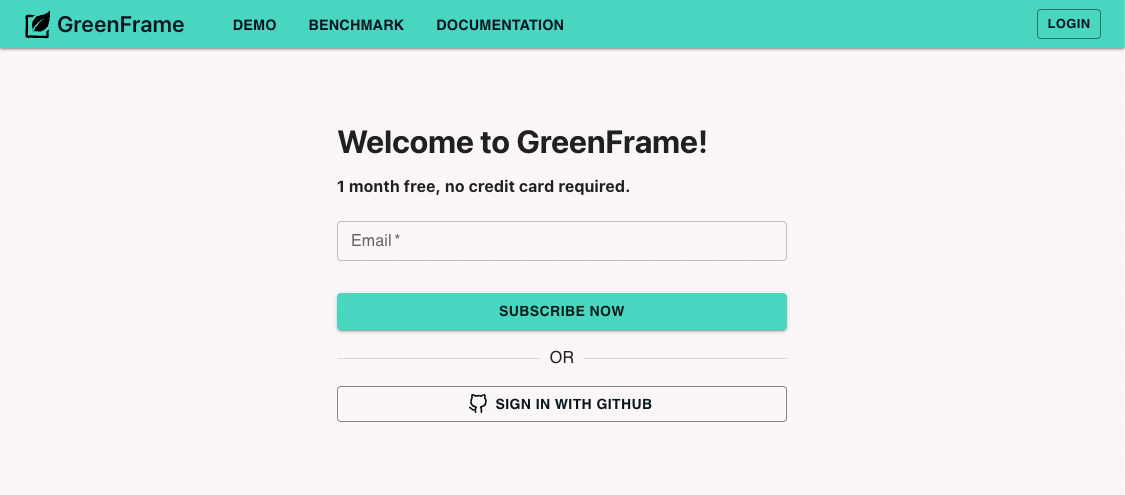
\includegraphics[width=0.9\textwidth]{imagenes/Greenframe_1.png}
\end{center}

Tras crear una cuenta gratuita (1 mes), puedes iniciar un proyecto y elegir
entre dos tipos de análisis: \textbf{"Single page"} y \textbf{"Full stack"}. El
tipo \textit{Single page} está pensado para medir el impacto ambiental de una
visita a una página web concreta, como por ejemplo una
\textbf{landing}\footnote{Página de aterrizaje web diseñada para recibir
  visitas y provocar una acción específica, como registrarse o comprar.} o una
página de inicio. Es ideal para casos sencillos y rápidos de analizar. Por otro
lado, la opción \textit{Full stack} permite definir escenarios más complejos,
simulando acciones del usuario en varias páginas e incluyendo la medición del
comportamiento del servidor (como contenedores Docker), ofreciendo una visión
más completa de la huella digital de toda la aplicación.

\begin{center}
  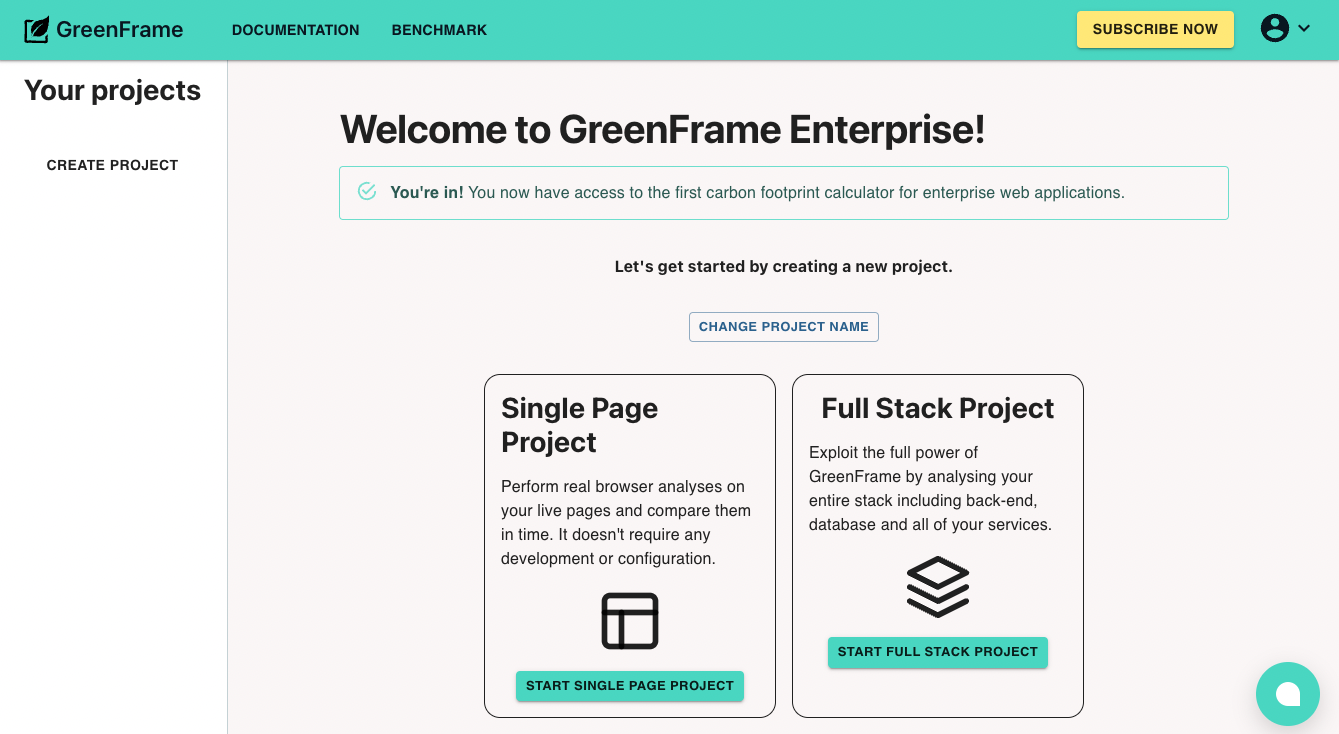
\includegraphics[width=0.9\textwidth]{imagenes/Greenframe_2.png}
\end{center}

Una vez que defines el tipo de proyecto e introduces la URL a analizar,
\textbf{GreenFrame simula tres visitas reales al sitio} usando un navegador en
la nube. Durante estas visitas registra múltiples métricas: uso de CPU, tráfico
de red, consumo de memoria y tiempo de carga. Esto le permite calcular de forma
más precisa las \textbf{emisiones estimadas de CO$_2$ equivalente (gCO$_2$e)}
que produce la interacción simulada.

\begin{center}
  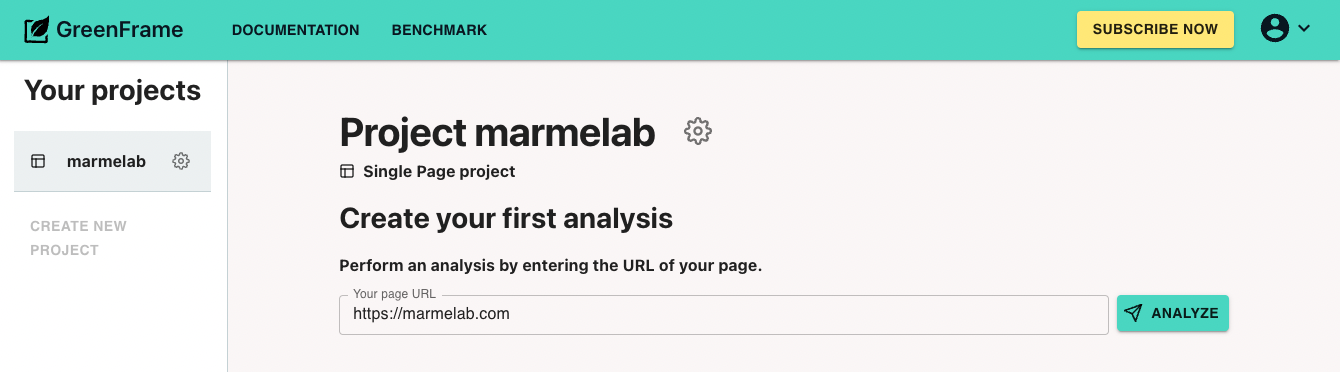
\includegraphics[width=0.9\textwidth]{imagenes/Greenframe_3.png}
\end{center}

\begin{center}
  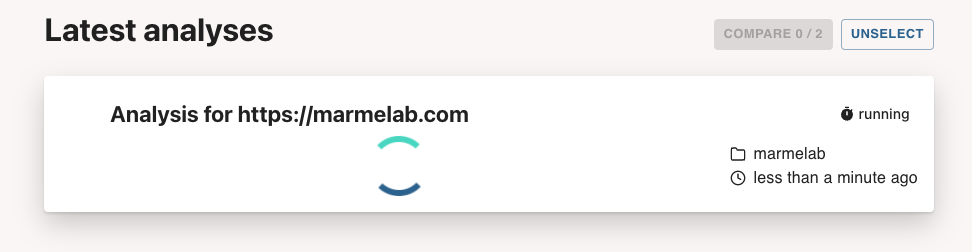
\includegraphics[width=0.9\textwidth]{imagenes/Greenframe_4.png}
\end{center}

Cuando el análisis finaliza (puede tardar unos minutos), se muestran los
resultados en una vista gráfica e interactiva. Se incluye un resumen con la
cantidad total de emisiones generadas y un \textbf{desglose por componentes y
  etapas del escenario}. Puedes examinar el comportamiento temporal de cada
componente (por ejemplo, el navegador), accediendo a una línea de tiempo que
detalla cómo y cuándo se generaron las emisiones durante la visita.

\begin{center}
  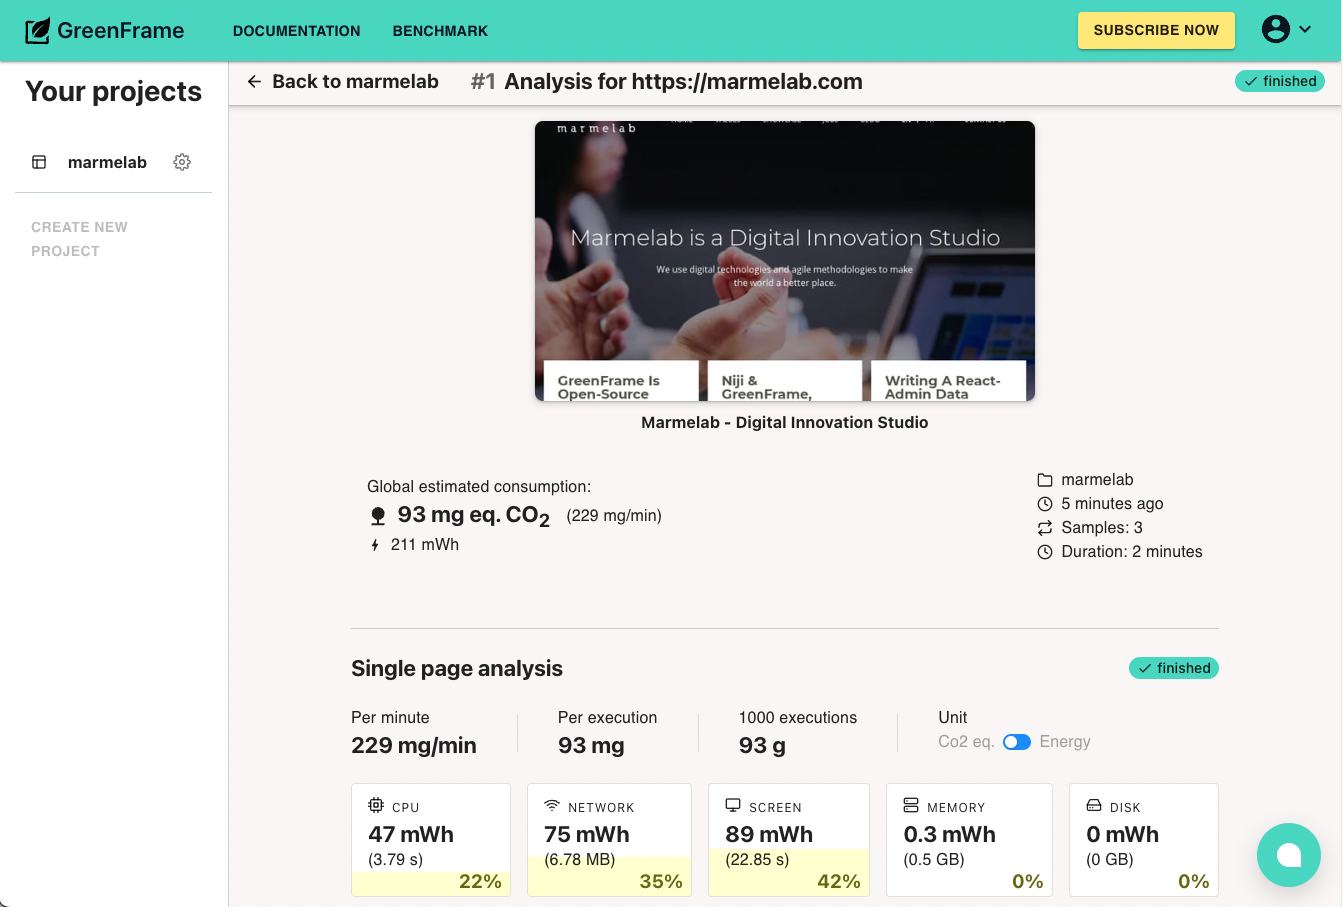
\includegraphics[width=0.9\textwidth]{imagenes/Greenframe_5.png}
\end{center}

\begin{center}
  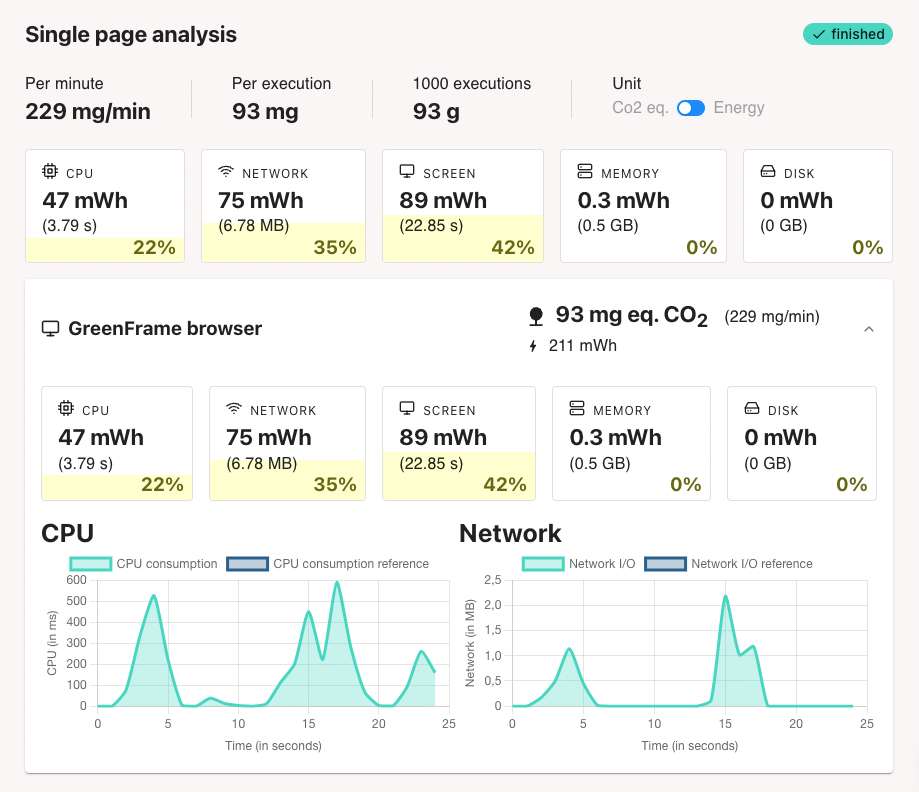
\includegraphics[width=0.9\textwidth]{imagenes/Greenframe_6.png}
\end{center}

Además, GreenFrame permite comparar diferentes análisis realizados sobre la
misma página o en distintas versiones del sitio. Esto es útil para evaluar si
los cambios en el código o contenido han reducido (o aumentado) el impacto
ambiental. El sistema te avisa si las diferencias entre análisis son mínimas y
podrían no ser significativas.

\begin{center}
  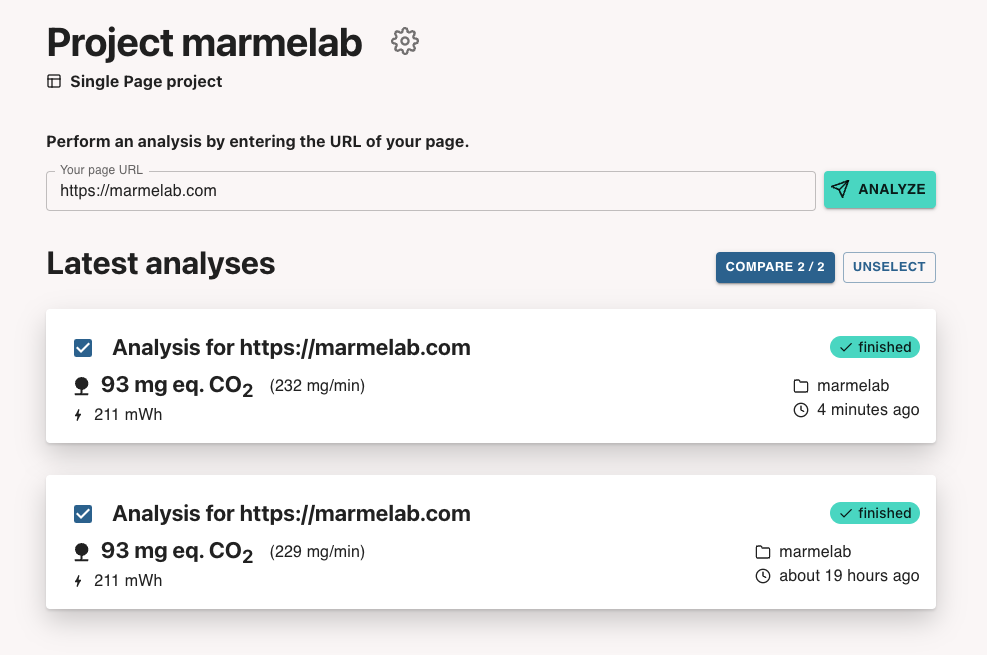
\includegraphics[width=0.9\textwidth]{imagenes/Greenframe_7.png}
\end{center}

\begin{center}
  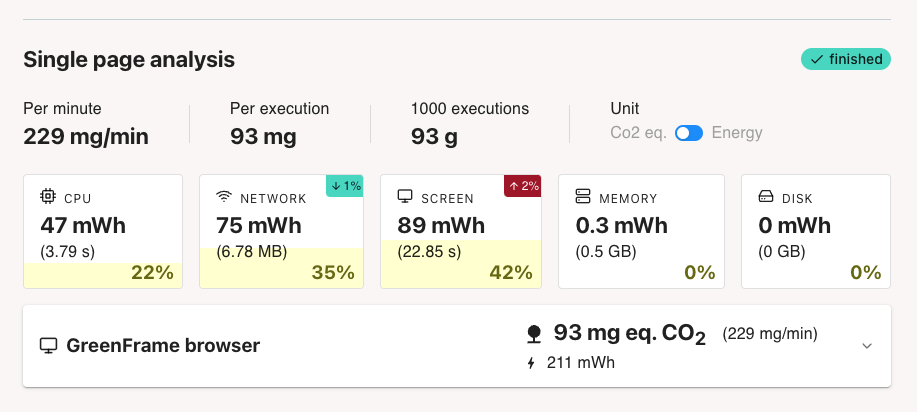
\includegraphics[width=0.9\textwidth]{imagenes/Greenframe_8.png}
\end{center}

Además, puedes usar \textbf{GreenFrame desde la terminal con su CLI}, o
integrarlo en un \textbf{pipeline de integración continua
  (CI}\footnote{(Continuous Integration) Técnica de desarrollo que automatiza la
  integración de código mediante pruebas continuas.}) para análisis
automatizados. Estas opciones son más potentes para desarrolladores que buscan
incorporar la sostenibilidad en sus flujos de trabajo.

\textbf{Puntos fuertes:}
\begin{itemize}
  \item \textbf{Alta precisión y detalle}: mide múltiples métricas (CPU, memoria, red, disco, PUE), diferenciando tráfico local y externo.
  \item \textbf{Pensado para desarrolladores}: comparativas entre versiones y páginas específicas.
  \item \textbf{Soporta distintos niveles de análisis}: desde páginas individuales hasta aplicaciones completas (\textit{full-stack}).
  \item \textbf{Integración CI/CD}: integración con GitHub para evitar merges si se supera un umbral de emisiones.
  \item \textbf{Modelo validado científicamente}: desarrollado con el CNRS, transparente en metodología general.
\end{itemize}

\textbf{Puntos débiles:}
\begin{itemize}
  \item \textbf{Modelo parcialmente cerrado}: la conversión a energía y CO$_2$ no es completamente transparente (algunos elementos son secretos comerciales).
  \item \textbf{Limitaciones en versión gratuita}: no incluye almacenamiento histórico ni visualización temporal; requiere conocimientos técnicos para usar la CLI.
  \item \textbf{No modela interacciones largas}: se centra en visitas individuales, sin simular sesiones prolongadas.
  \item \textbf{Web UI completa solo en plan Enterprise}: requiere suscripción de pago
        (12€/usuario/mes).
  \item \textbf{Curva de aprendizaje}: uso de CLI y Playwright implica mayor complejidad técnica.
\end{itemize}

\section*{\textbf{Website Carbon Calculator}}

\url{https://www.websitecarbon.com/}

\url{https://www.websitecarbon.com/how-does-it-work/}

\textbf{Website Carbon Calculator} es una herramienta online gratuita que estima la huella de carbono de un sitio web analizando factores como el peso de la página, los recursos cargados, el tipo de contenido y la localización del servidor. Proporciona una puntuación energética (de la \textbf{A a la G}), una estimación de emisiones por visita y recomendaciones prácticas para mejorar la eficiencia.

Está pensada para facilitar una primera \textbf{auditoría}\footnote{Evaluación
  sistemática de una página web para determinar su eficiencia energética y huella
  digital.} accesible y sin conocimientos técnicos previos, siendo ideal para
usuarios no técnicos, diseñadores web y campañas de sensibilización. También
ofrece una \textbf{API REST}\footnote{Interfaz de programación que permite
  acceder a los servicios del sitio mediante solicitudes HTTP automatizadas.}
para integraciones automatizadas.

La forma más sencilla y recomendada de utilizar Website Carbon Calculator es a
través de su interfaz web.

\begin{center}
  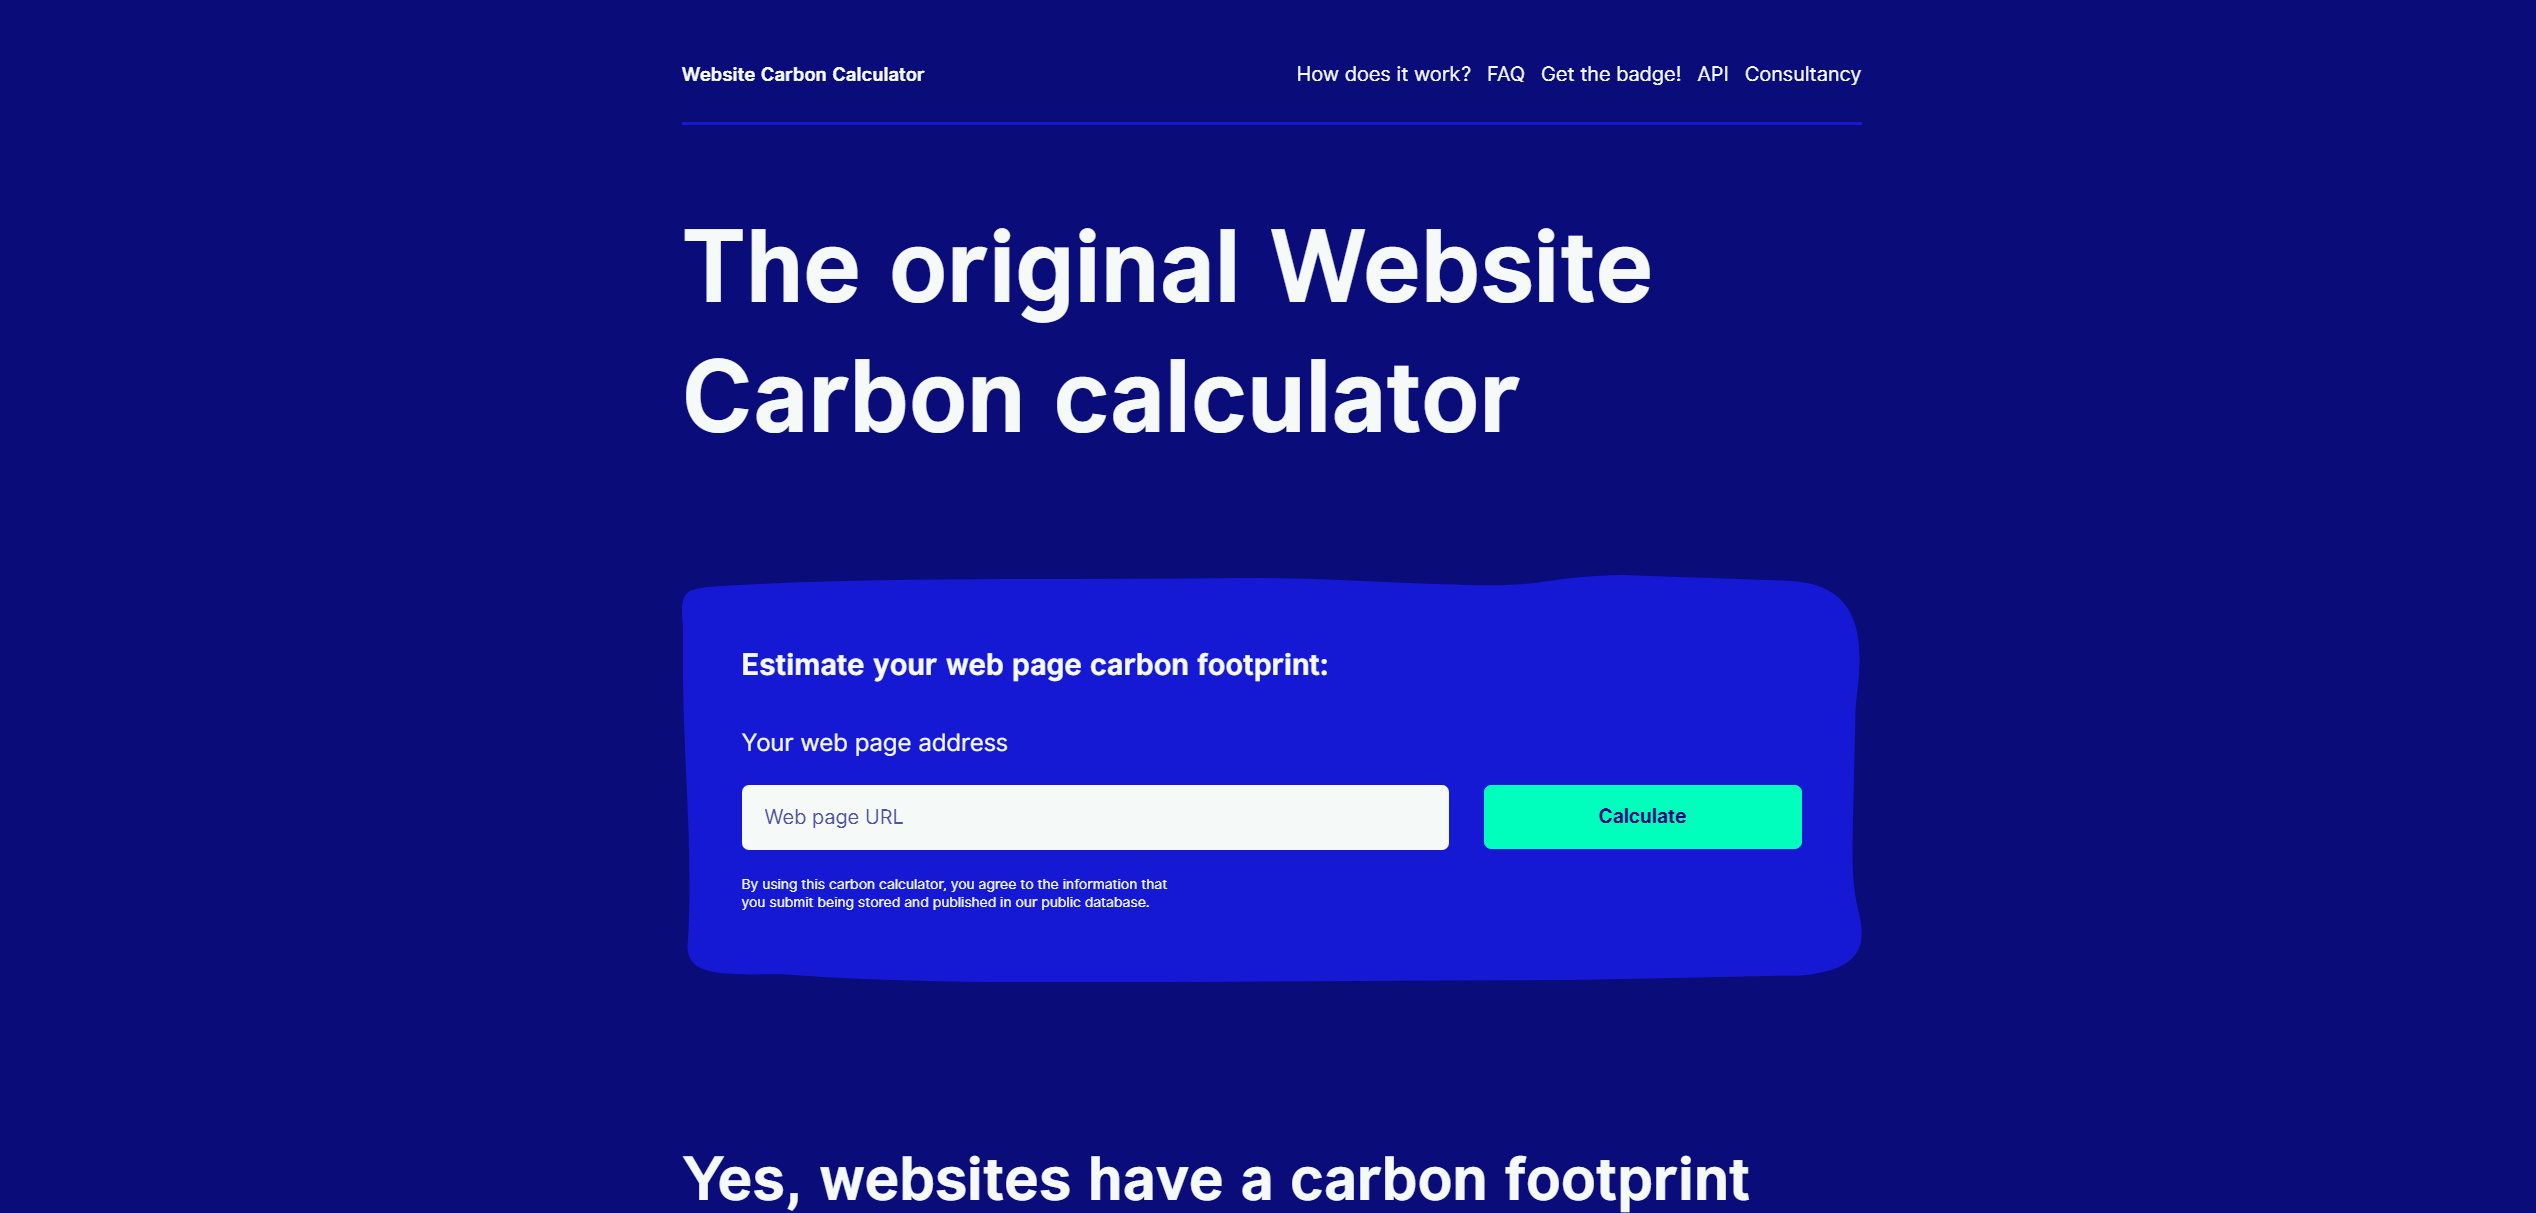
\includegraphics[width=0.7\textwidth]{imagenes/WCC_1.png}
\end{center}

Al introducir la URL del sitio web a analizar, la herramienta realiza las
siguientes acciones:

\begin{itemize}
  \item Mide el volumen de datos transferidos al cargar la página.
  \item Aplica un \textbf{factor de energía promedio por byte}\footnote{Estimación de
          energía consumida al transferir datos en internet, considerando red, servidores
          y dispositivos.}, considerando el consumo en el dispositivo del usuario, la red
        y el centro de datos.
  \item Consulta la base de datos de la \textbf{Green Web
          Foundation}\footnote{Organización que mantiene una base de datos sobre si los
          proveedores usan energía renovable.} para saber si el proveedor de alojamiento
        usa energía renovable.
  \item Convierte el consumo energético estimado (en kWh) en emisiones de CO$_2$e
        utilizando factores de conversión basados en la fuente de energía.
\end{itemize}

El resultado del análisis incluye:

\begin{itemize}
  \item \textbf{Emisiones estimadas por visita} (en gCO$_2$e).
  \item Comparación con el \textbf{promedio global} (\textasciitilde0.8
        gCO$_2$e/vista).
  \item \textbf{Porcentaje ''cleanerThan''}\footnote{Métrica que indica el porcentaje de sitios web más contaminantes que el analizado.}: indica qué proporción de sitios analizados son más contaminantes que el tuyo.
  \item Estimación anual de emisiones basada en el número de visitas.
\end{itemize}

\begin{center}
  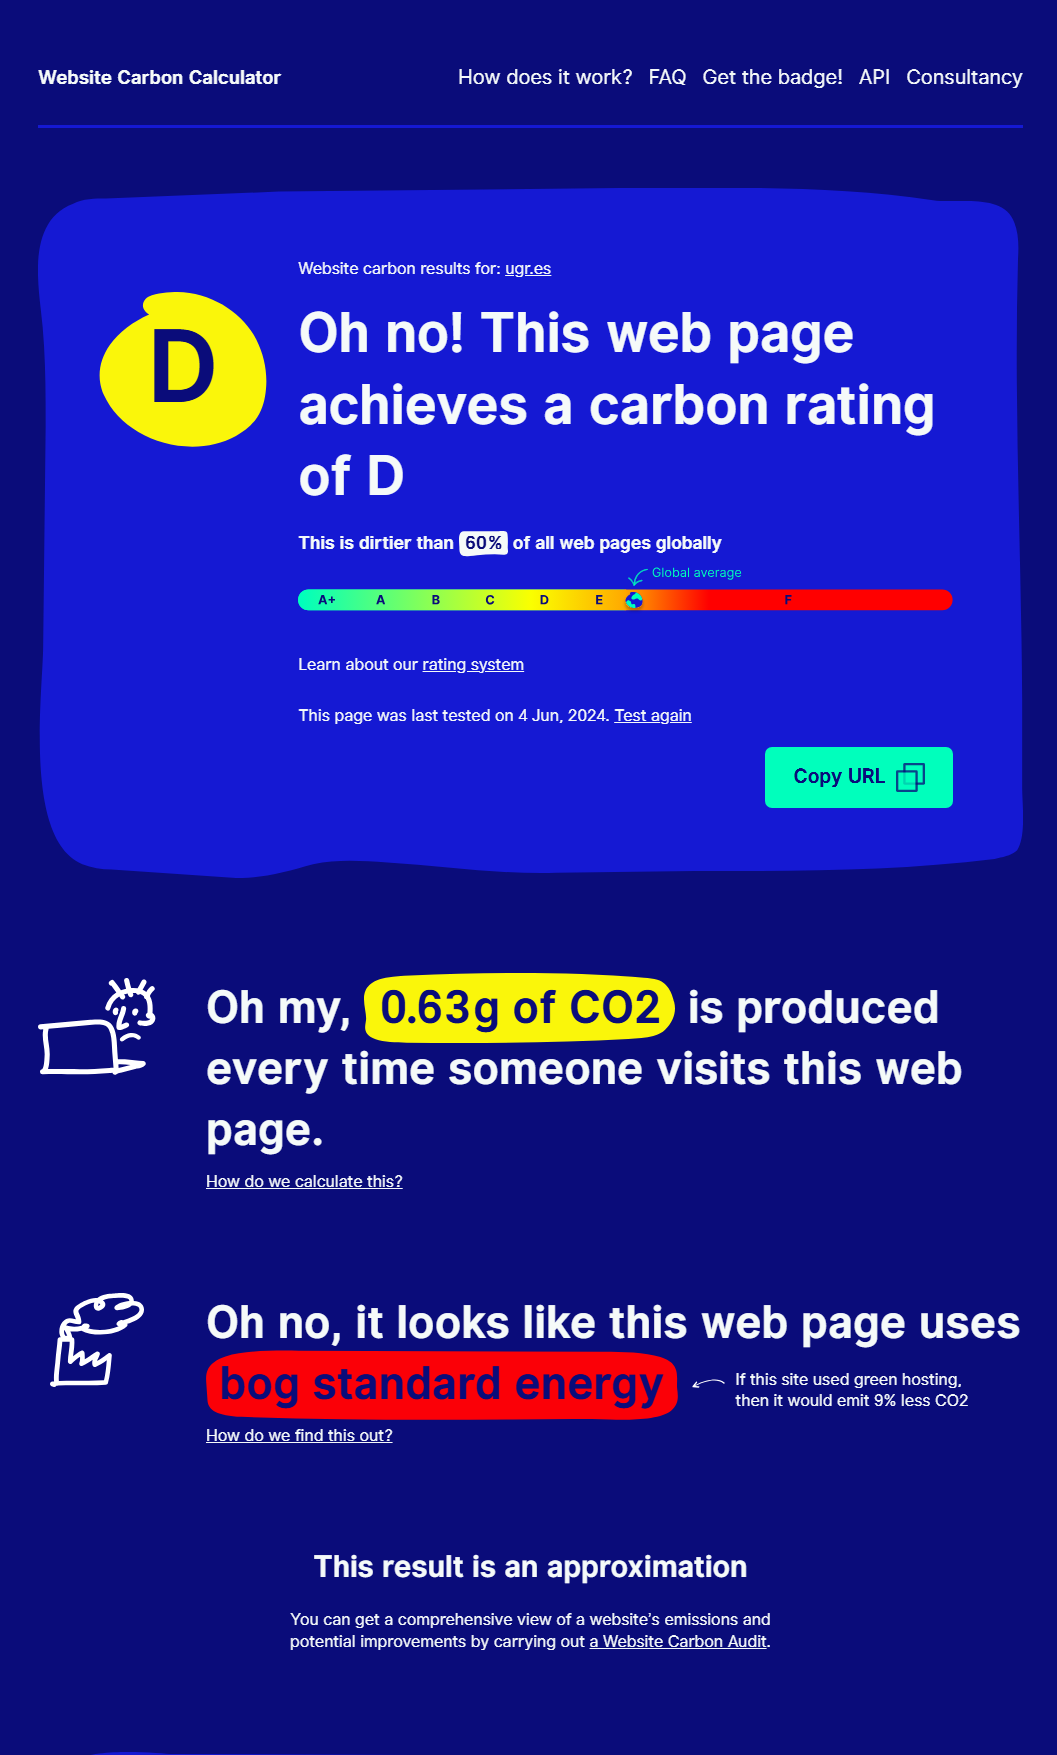
\includegraphics[width=0.7\textwidth]{imagenes/WCC_2.png}
\end{center}

\begin{center}
  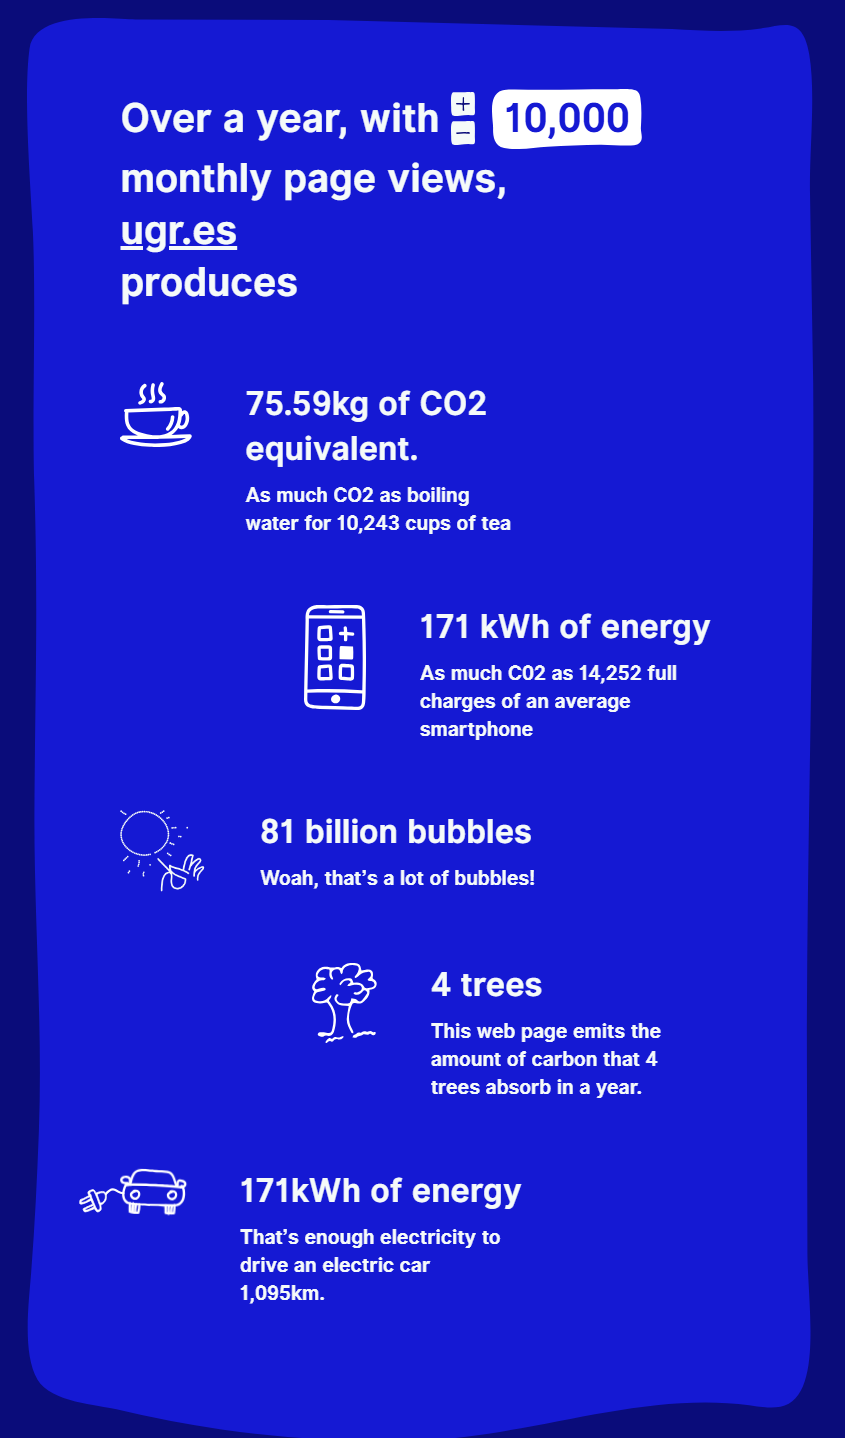
\includegraphics[width=0.7\textwidth]{imagenes/WCC_3.png}
\end{center}

\textbf{Puntos fuertes:}
\begin{itemize}
  \item \textbf{Extremadamente accesible}: no requiere conocimientos técnicos.
  \item \textbf{Rápido y visual}: análisis en pocos segundos con resultados claros.
  \item \textbf{Comparación global}: útil para campañas de concienciación y benchmarking.
  \item \textbf{Gratuito y abierto}: interfaz sin coste y documentación disponible.
  \item \textbf{API disponible}: permite automatizar análisis desde scripts o plataformas externas.
\end{itemize}

\textbf{Puntos débiles:}
\begin{itemize}
  \item \textbf{Modelo simplificado}: no mide interacciones complejas ni escenarios completos.
  \item \textbf{Menor precisión técnica}: basado en estimaciones generales, no analiza procesos del lado servidor.
  \item \textbf{No incluye comportamiento dinámico}: ignora scripts posteriores a la carga inicial.
  \item \textbf{No distingue tráfico local/internacional}: aplica valores promedio que pueden no reflejar la realidad específica.
  \item \textbf{Sin personalización ni históricos}: cada análisis es aislado, sin seguimiento temporal.
\end{itemize}

\section*{\textbf{Ecograder}}

\url{https://ecograder.com/}

\textbf{Ecograder} es una herramienta gratuita que analiza la sostenibilidad de sitios web desde una perspectiva técnica y ambiental. Proporciona una puntuación de 1 a 100 basada en criterios como eficiencia del frontend, peso de la página, experiencia de usuario (UX) y uso de hosting sostenible. Utiliza el script \textbf{CO2.js}\footnote{Biblioteca de código abierto que estima las emisiones de carbono de una página web basándose en cuatro áreas: dispositivo, red, servidor y hardware.} para calcular las emisiones estimadas de carbono.

Es ideal para consultoras, desarrolladores web y diseñadores que buscan evaluar
y mejorar la eficiencia ambiental de sus sitios de forma rápida, sin necesidad
de configuración ni conocimientos avanzados.

Para usarlo solo necesitaremos entrar en su web \url{https://ecograder.com/} y
introducir la URL de la web que queremos analizar.

\begin{center}
  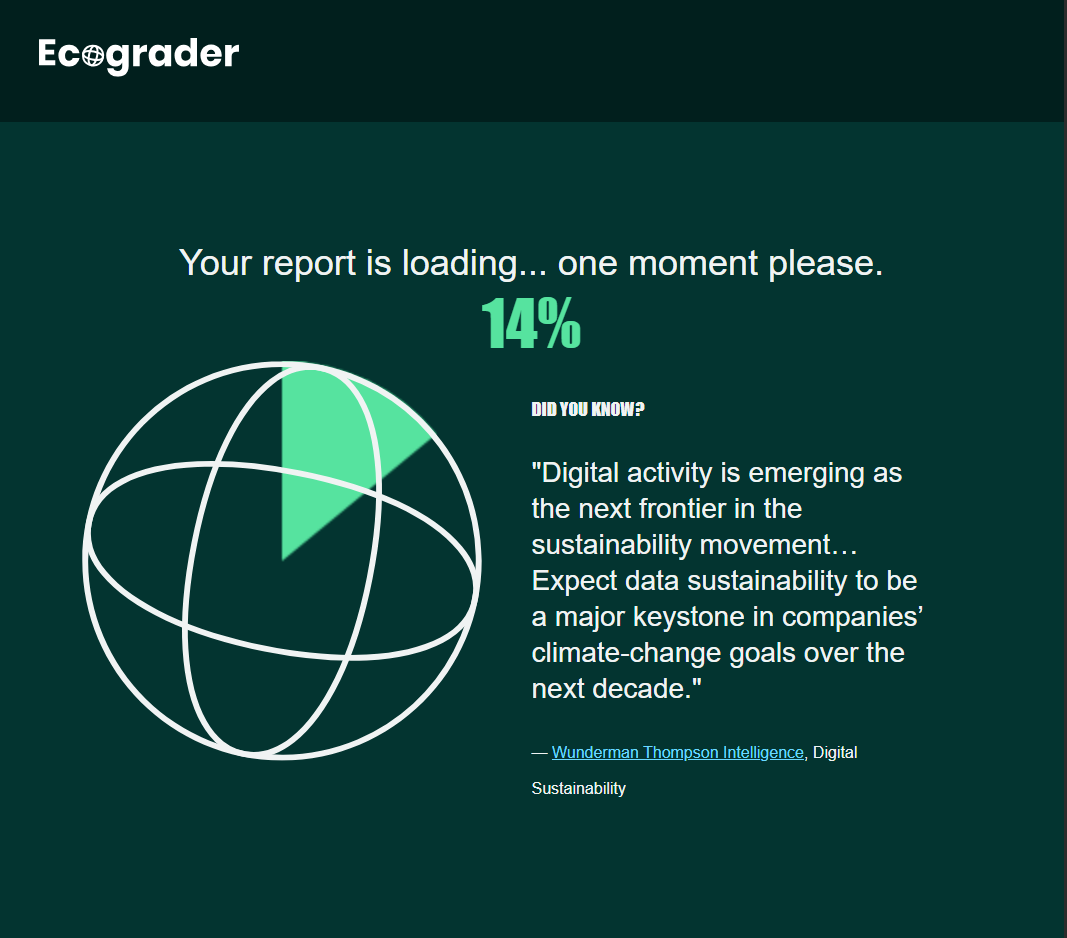
\includegraphics[width=0.9\textwidth]{imagenes/Ecograder_1.png}
\end{center}

ECOGrader lanzará un análisis que combina
\textbf{Lighthouse}\footnote{Herramienta automatizada de Google que audita el
  rendimiento, accesibilidad y buenas prácticas de páginas web.} y
\textbf{CO2.js} para estimar las emisiones de CO$_2$ equivalente (gCO$_2$e).
\textbf{CO2.js} calcula emisiones según cuatro segmentos: dispositivo de
usuario, red, centro de datos (usando datos de la red eléctrica regional, según
la \textbf{intensidad de carbono regional}) y producción de hardware. Además, integra datos de
intensidad de carbono por región y detecta si el sitio está alojado en un
proveedor "\textbf{hosting verde}"\footnote{Servicio de alojamiento web
  alimentado total o parcialmente por fuentes de energía renovables.}. Por su
parte, \textbf{Lighthouse} aporta métricas de rendimiento como "\textbf{First
  Contentful Paint (FCP)}"\footnote{Métrica de Lighthouse que mide el tiempo
  hasta que el primer contenido se renderiza en pantalla.} o "\textbf{Time to
  Interactive (TTI)}"\footnote{Métrica de Lighthouse que indica cuándo una página
  se vuelve completamente interactiva para el usuario.}, que ECOGrader adapta
para generar recomendaciones de optimización.

\begin{center}
  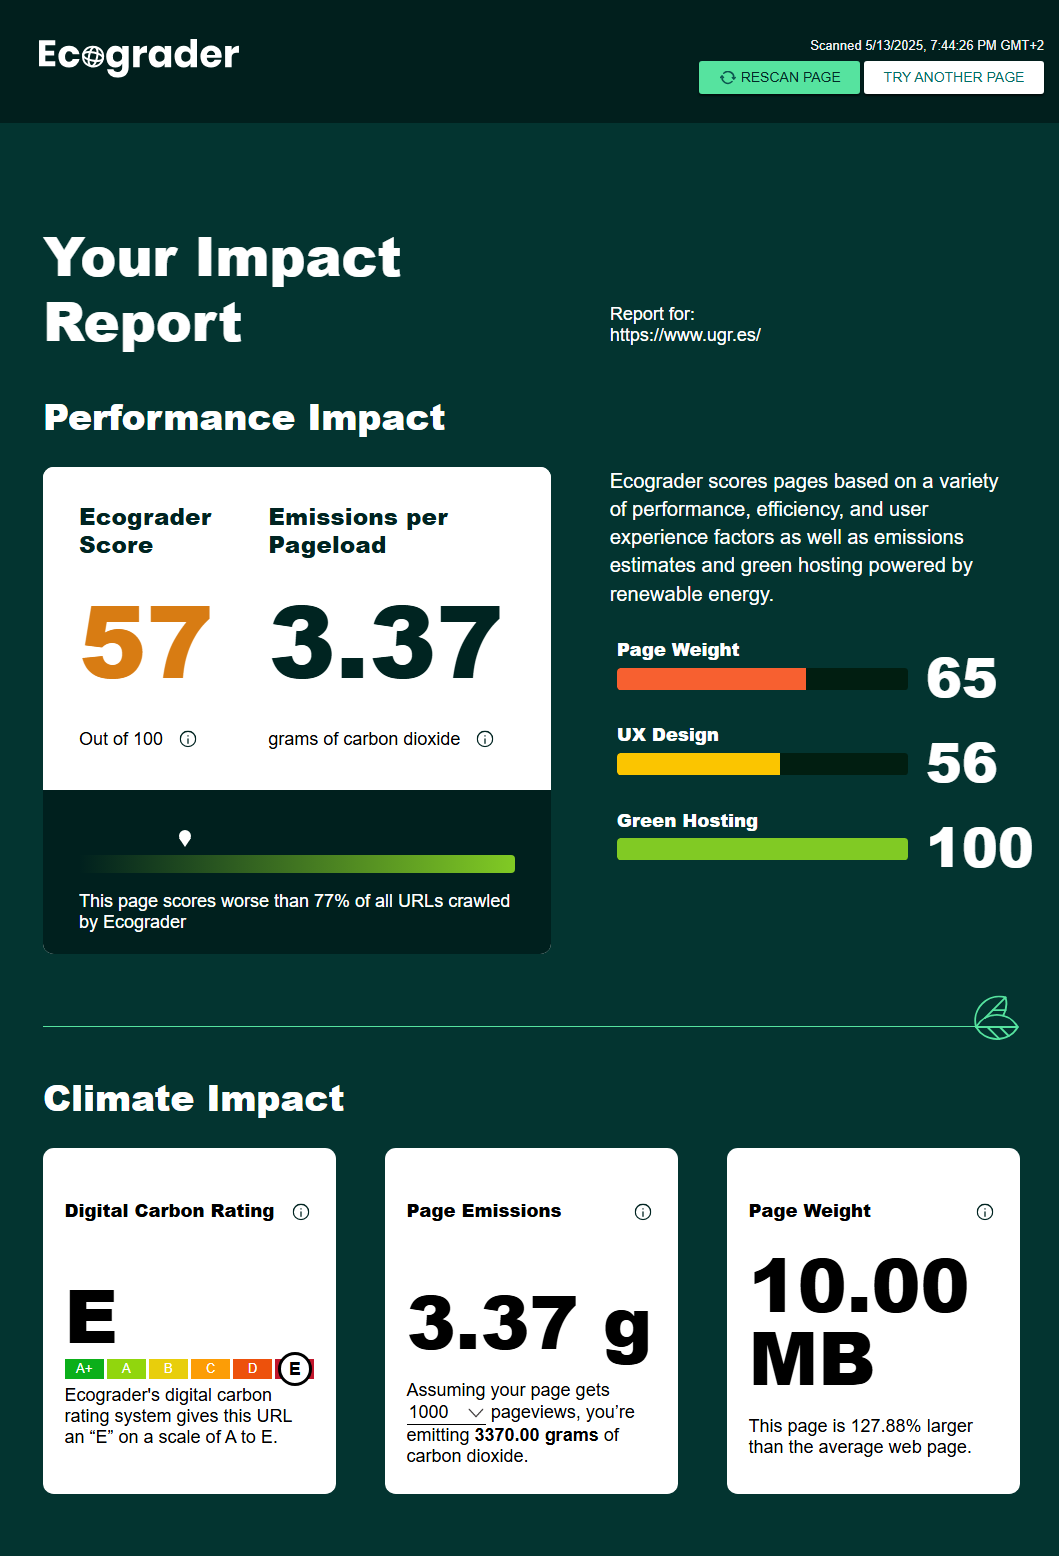
\includegraphics[width=0.9\textwidth]{imagenes/Ecograder_2.png}
\end{center}

\begin{center}
  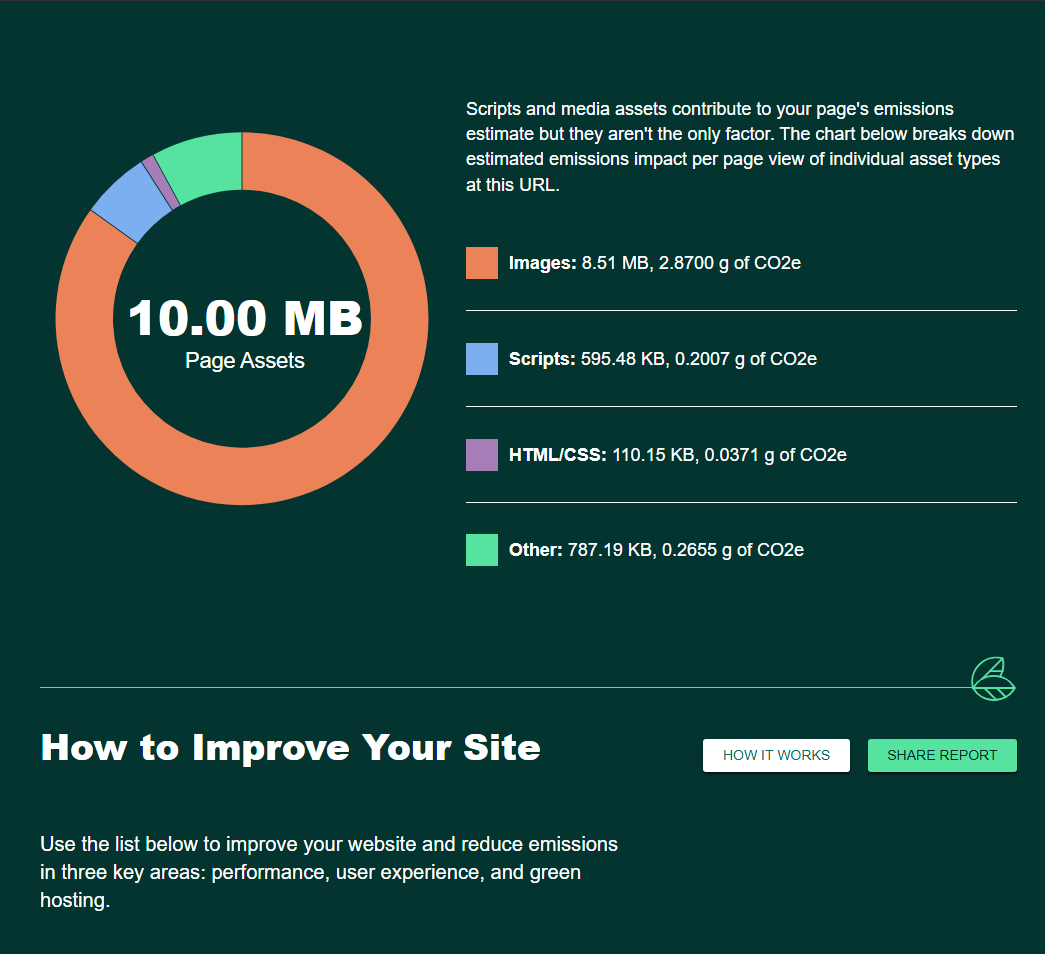
\includegraphics[width=0.9\textwidth]{imagenes/Ecograder_3.png}
\end{center}

\begin{center}
  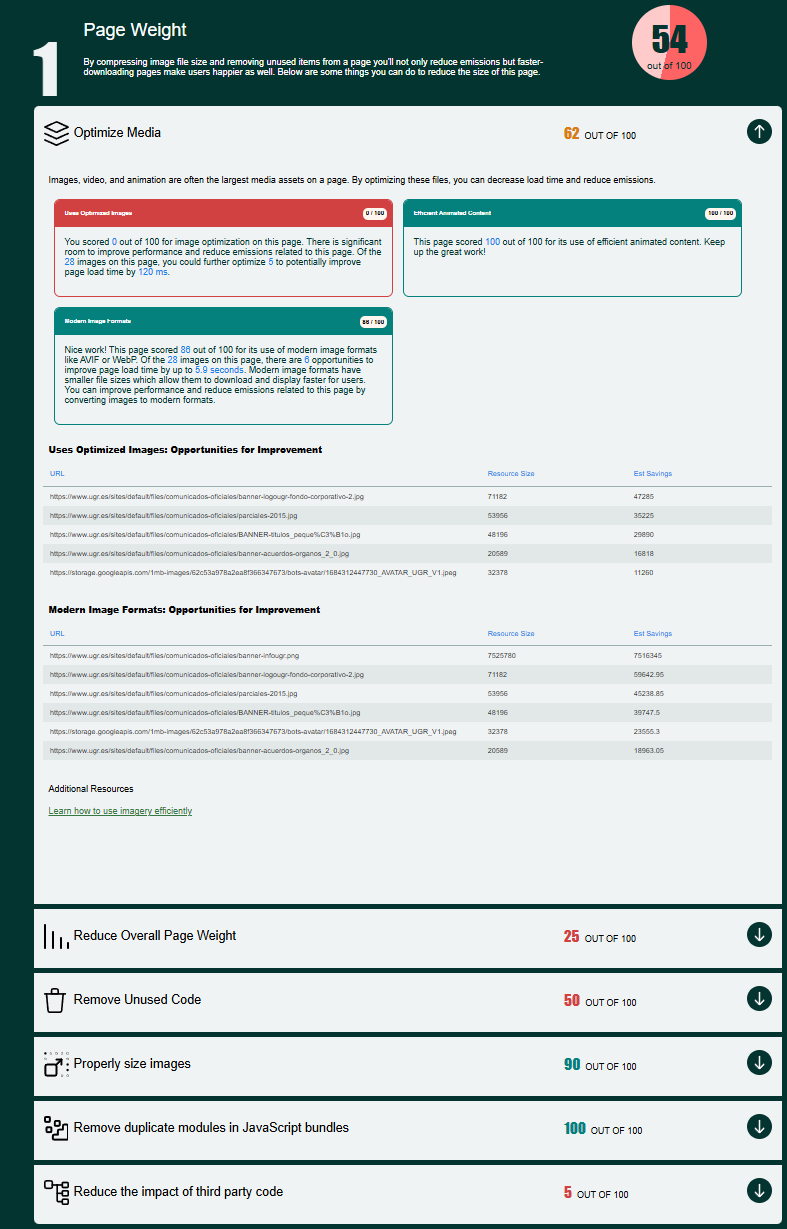
\includegraphics[width=0.9\textwidth]{imagenes/Ecograder_4.png}
\end{center}

\begin{center}
  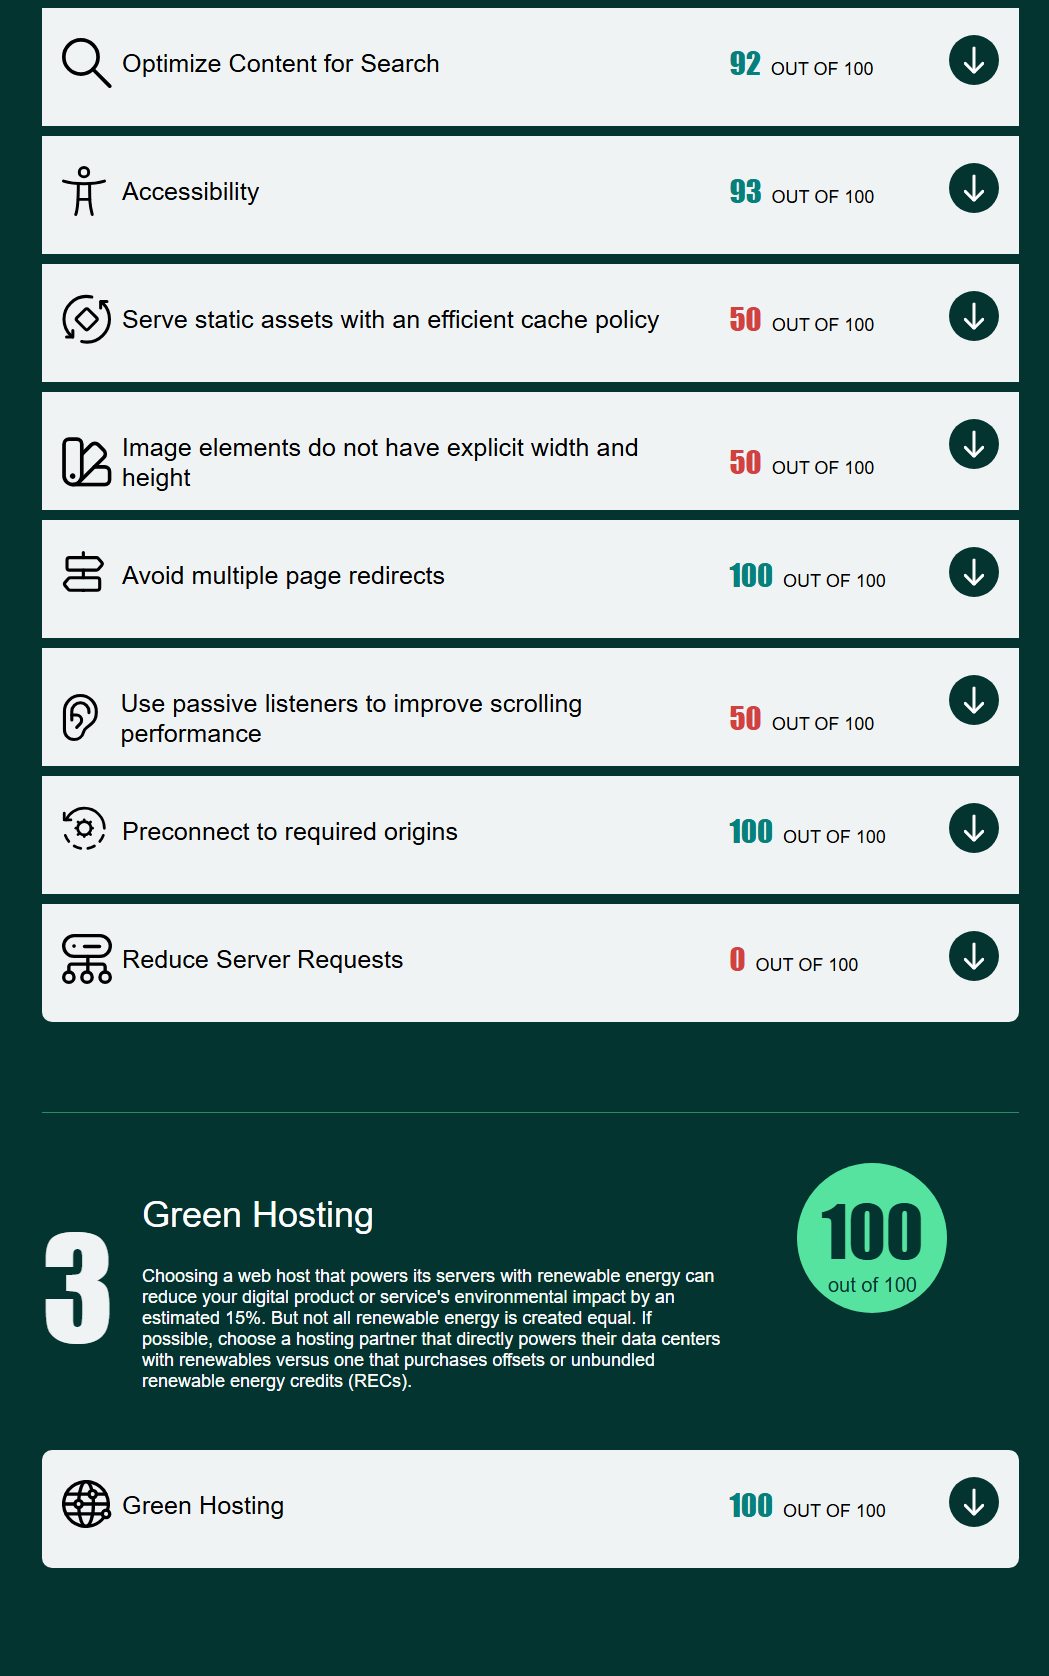
\includegraphics[width=0.9\textwidth]{imagenes/Ecograder_5.png}
\end{center}

\textbf{Puntos fuertes:}
\begin{itemize}
  \item \textbf{Interfaz visual e intuitiva}: muestra resultados desglosados por categoría (peso, UX, hosting), con gráficas y explicaciones claras.
  \item \textbf{Puntuación global (1–100)}: facilita la interpretación rápida del rendimiento ecológico de un sitio web.
  \item \textbf{Recomendaciones técnicas útiles}: incluye sugerencias concretas como minificar recursos, reducir llamadas HTTP, o cambiar a un proveedor de hosting verde.
  \item \textbf{Basado en CO2.js}: ofrece transparencia y confianza al usar una metodología reconocida y de código abierto para estimar emisiones.
  \item \textbf{Acceso instantáneo}: sólo requiere introducir una URL para obtener el análisis, sin necesidad de registro ni instalación.
  \item \textbf{Evaluación multidimensional}\footnote{Análisis que contempla varios factores técnicos y ambientales, como eficiencia del código, UX, tamaño de archivos y uso de energía sostenible.}: considera tanto eficiencia técnica como prácticas sostenibles (energía renovable, peso de recursos, etc.).
\end{itemize}

\textbf{Puntos débiles:}
\begin{itemize}
  \item \textbf{Limitado al frontend}: no evalúa consumo energético de servidores, APIs, bases de datos u otros elementos backend, solo hace una estimación del consumo energético basada en el tráfico de red y la intensidad de carbono regional.
  \item \textbf{Resultados poco estables}: las puntuaciones pueden variar entre análisis consecutivos debido a cambios dinámicos en el sitio o actualizaciones de la propia herramienta.
  \item \textbf{Sin simulaciones de usuario}: no permite crear escenarios personalizados ni medir la huella en flujos de interacción reales.
  \item \textbf{No guarda históricos}: no permite comparar resultados a lo largo del tiempo ni registrar progresos entre versiones.
  \item \textbf{Un solo análisis por vez}: no se pueden evaluar varias páginas simultáneamente desde la interfaz actual ya que aún no cuentan con una API.
\end{itemize}

\section*{\textbf{CodeCarbon}}

\url{https://codecarbon.io/}

\url{https://mlco2.github.io/codecarbon/}

\textbf{CodeCarbon} es una biblioteca ligera de Python diseñada para estimar las emisiones de CO$_2$ asociadas a la ejecución de scripts y procesos computacionales. Calcula el consumo energético de CPU, GPU y RAM, y convierte estos datos en emisiones aproximadas según la \textbf{intensidad de carbono regional} de la región geográfica donde se ejecuta el código. Se integra fácilmente mediante \textbf{decoradores}\footnote{Función en Python que modifica el comportamiento de otra función o método.} o \textbf{gestores de contexto}\footnote{Estructura que gestiona recursos con `with` en Python.}.

Es una solución ideal para proyectos de ciencia de datos, *machine learning* o
cualquier \textbf{pipeline}\footnote{Secuencia automatizada de procesos o
  tareas en datos o código.} Python que quiera monitorizar su huella de carbono.

Para poder usarlo en nuestros proyectos instalaremos el paquete de Python
usando los gestores de paquete \textbf{pip}\footnote{Herramienta para instalar
  y gestionar paquetes de Python.} o \textbf{conda}\footnote{Gestor de entornos y
  paquetes, popular en ciencia de datos.}:

\begin{tcolorbox}[colback=codebackground, colframe=codeborder, boxrule=0.8pt, arc=0mm, boxsep=5pt, left=5pt, right=5pt, top=5pt, bottom=5pt]
  \begin{lstlisting}[language=bash]
    pip install codecarbon
  \end{lstlisting}
\end{tcolorbox}

Tras esto, usando el comando

\begin{tcolorbox}[colback=codebackground, colframe=codeborder, boxrule=0.8pt, arc=0mm, boxsep=5pt, left=5pt, right=5pt, top=5pt, bottom=5pt]
  \begin{lstlisting}[language=bash]
    codecarbon config
  \end{lstlisting}
\end{tcolorbox}

se nos guiará a la hora de crear el archivo de configuración de nuestro
proyecto, en el que indicaremos datos como la región o si este se está
ejecutando en la nube.

A continuación ya podemos monitorear las emisiones de nuestro equipo sin
cambiar el código con:

\begin{tcolorbox}[colback=codebackground, colframe=codeborder, boxrule=0.8pt, arc=0mm, boxsep=5pt, left=5pt, right=5pt, top=5pt, bottom=5pt]
  \begin{lstlisting}[language=bash]
    codecarbon monitor
  \end{lstlisting}
\end{tcolorbox}

El cual enviará la información a una \textbf{API} alojada en
"localhost:8008".

\textbf{CodeCarbon} también permite medir emisiones usando un objeto \texttt{EmissionsTracker} con \texttt{start()} y \texttt{stop()}, ideal para bloques amplios de código:

\begin{tcolorbox}[colback=codebackground, colframe=codeborder, boxrule=0.8pt, arc=0mm, boxsep=5pt, left=5pt, right=5pt, top=5pt, bottom=5pt]
  \begin{lstlisting}[language=bash]
    from codecarbon import EmissionsTracker
    tracker = EmissionsTracker()
    tracker.start()
    try:
      #Codigo intensivo en computo aqui
      _ = 1 + 1
    finally:
      tracker.stop()
  \end{lstlisting}
\end{tcolorbox}

Y para secciones específicas puedes usar tareas con \texttt{start\_task()} /
\texttt{stop\_task()}:

\begin{tcolorbox}[colback=codebackground, colframe=codeborder, boxrule=0.8pt, arc=0mm, boxsep=5pt, left=5pt, right=5pt, top=5pt, bottom=5pt]
  \begin{lstlisting}[language=bash]
    try:
      tracker = EmissionsTracker(project_name="bert_inference", measure_power_secs=10)
      tracker.start_task("load dataset")
      dataset = load_dataset("imdb", split="test")
      imdb_emissions = tracker.stop_task()
      tracker.start_task("build model")
      model = build_model()
      model_emissions = tracker.stop_task()
    finally:
      _ = tracker.stop()
  \end{lstlisting}
\end{tcolorbox}

Otra opción es el uso como \textbf{gestor de contexto\textsuperscript{3}}:

\begin{tcolorbox}[colback=codebackground, colframe=codeborder, boxrule=0.8pt, arc=0mm, boxsep=5pt, left=5pt, right=5pt, top=5pt, bottom=5pt]
  \begin{lstlisting}[language=bash]
  from codecarbon import EmissionsTracker

  with EmissionsTracker() as tracker:
    # Codigo intensivo aqui
  \end{lstlisting}
\end{tcolorbox}

Y finalmente, si tu código está en una función, puedes decorarla con
\texttt{@track\_emissions}:

\begin{tcolorbox}[colback=codebackground, colframe=codeborder, boxrule=0.8pt, arc=0mm, boxsep=5pt, left=5pt, right=5pt, top=5pt, bottom=5pt]
  \begin{lstlisting}[language=bash]
  from codecarbon import track_emissions

  @track_emissions
  def training_loop():
    # Codigo de entrenamiento intensivo aqui
  \end{lstlisting}
\end{tcolorbox}

Además, dispones de dos formas de visualizar los datos recopilados:

\textbf{Offline}, con la herramienta \texttt{carbonboard}:

\begin{tcolorbox}[colback=codebackground, colframe=codeborder, boxrule=0.8pt, arc=0mm, boxsep=5pt, left=5pt, right=5pt, top=5pt, bottom=5pt]
  \begin{lstlisting}[language=bash]
  carbonboard --filepath="examples/emissions.csv" --port=3333
  \end{lstlisting}
\end{tcolorbox}

\begin{center}
  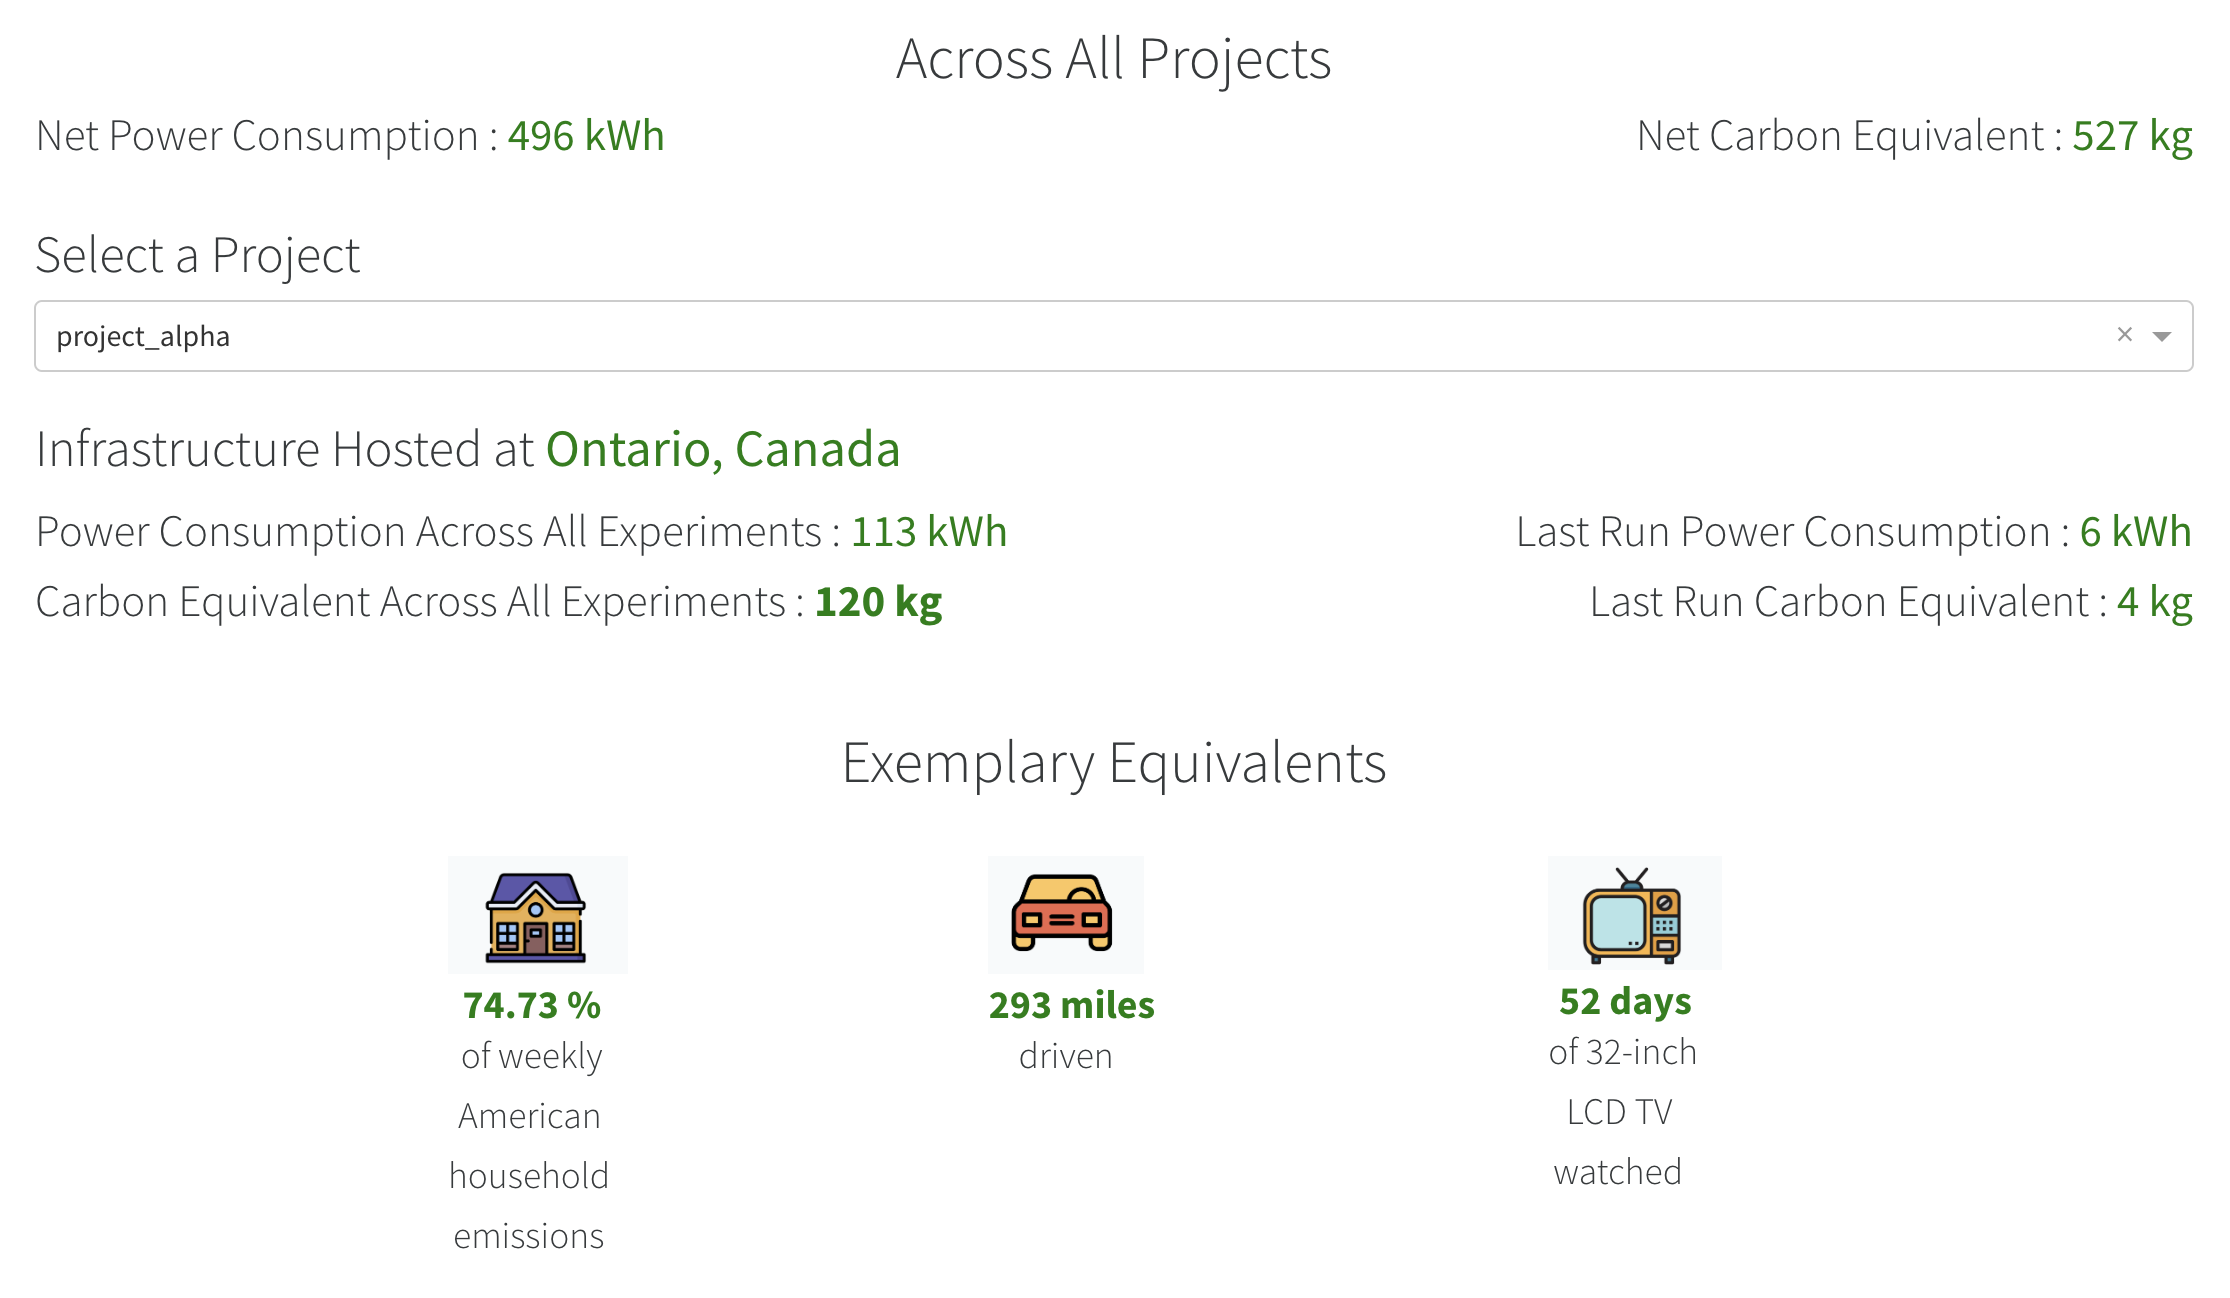
\includegraphics[width=0.9\textwidth]{imagenes/CC_1.png}
\end{center}

\begin{center}
  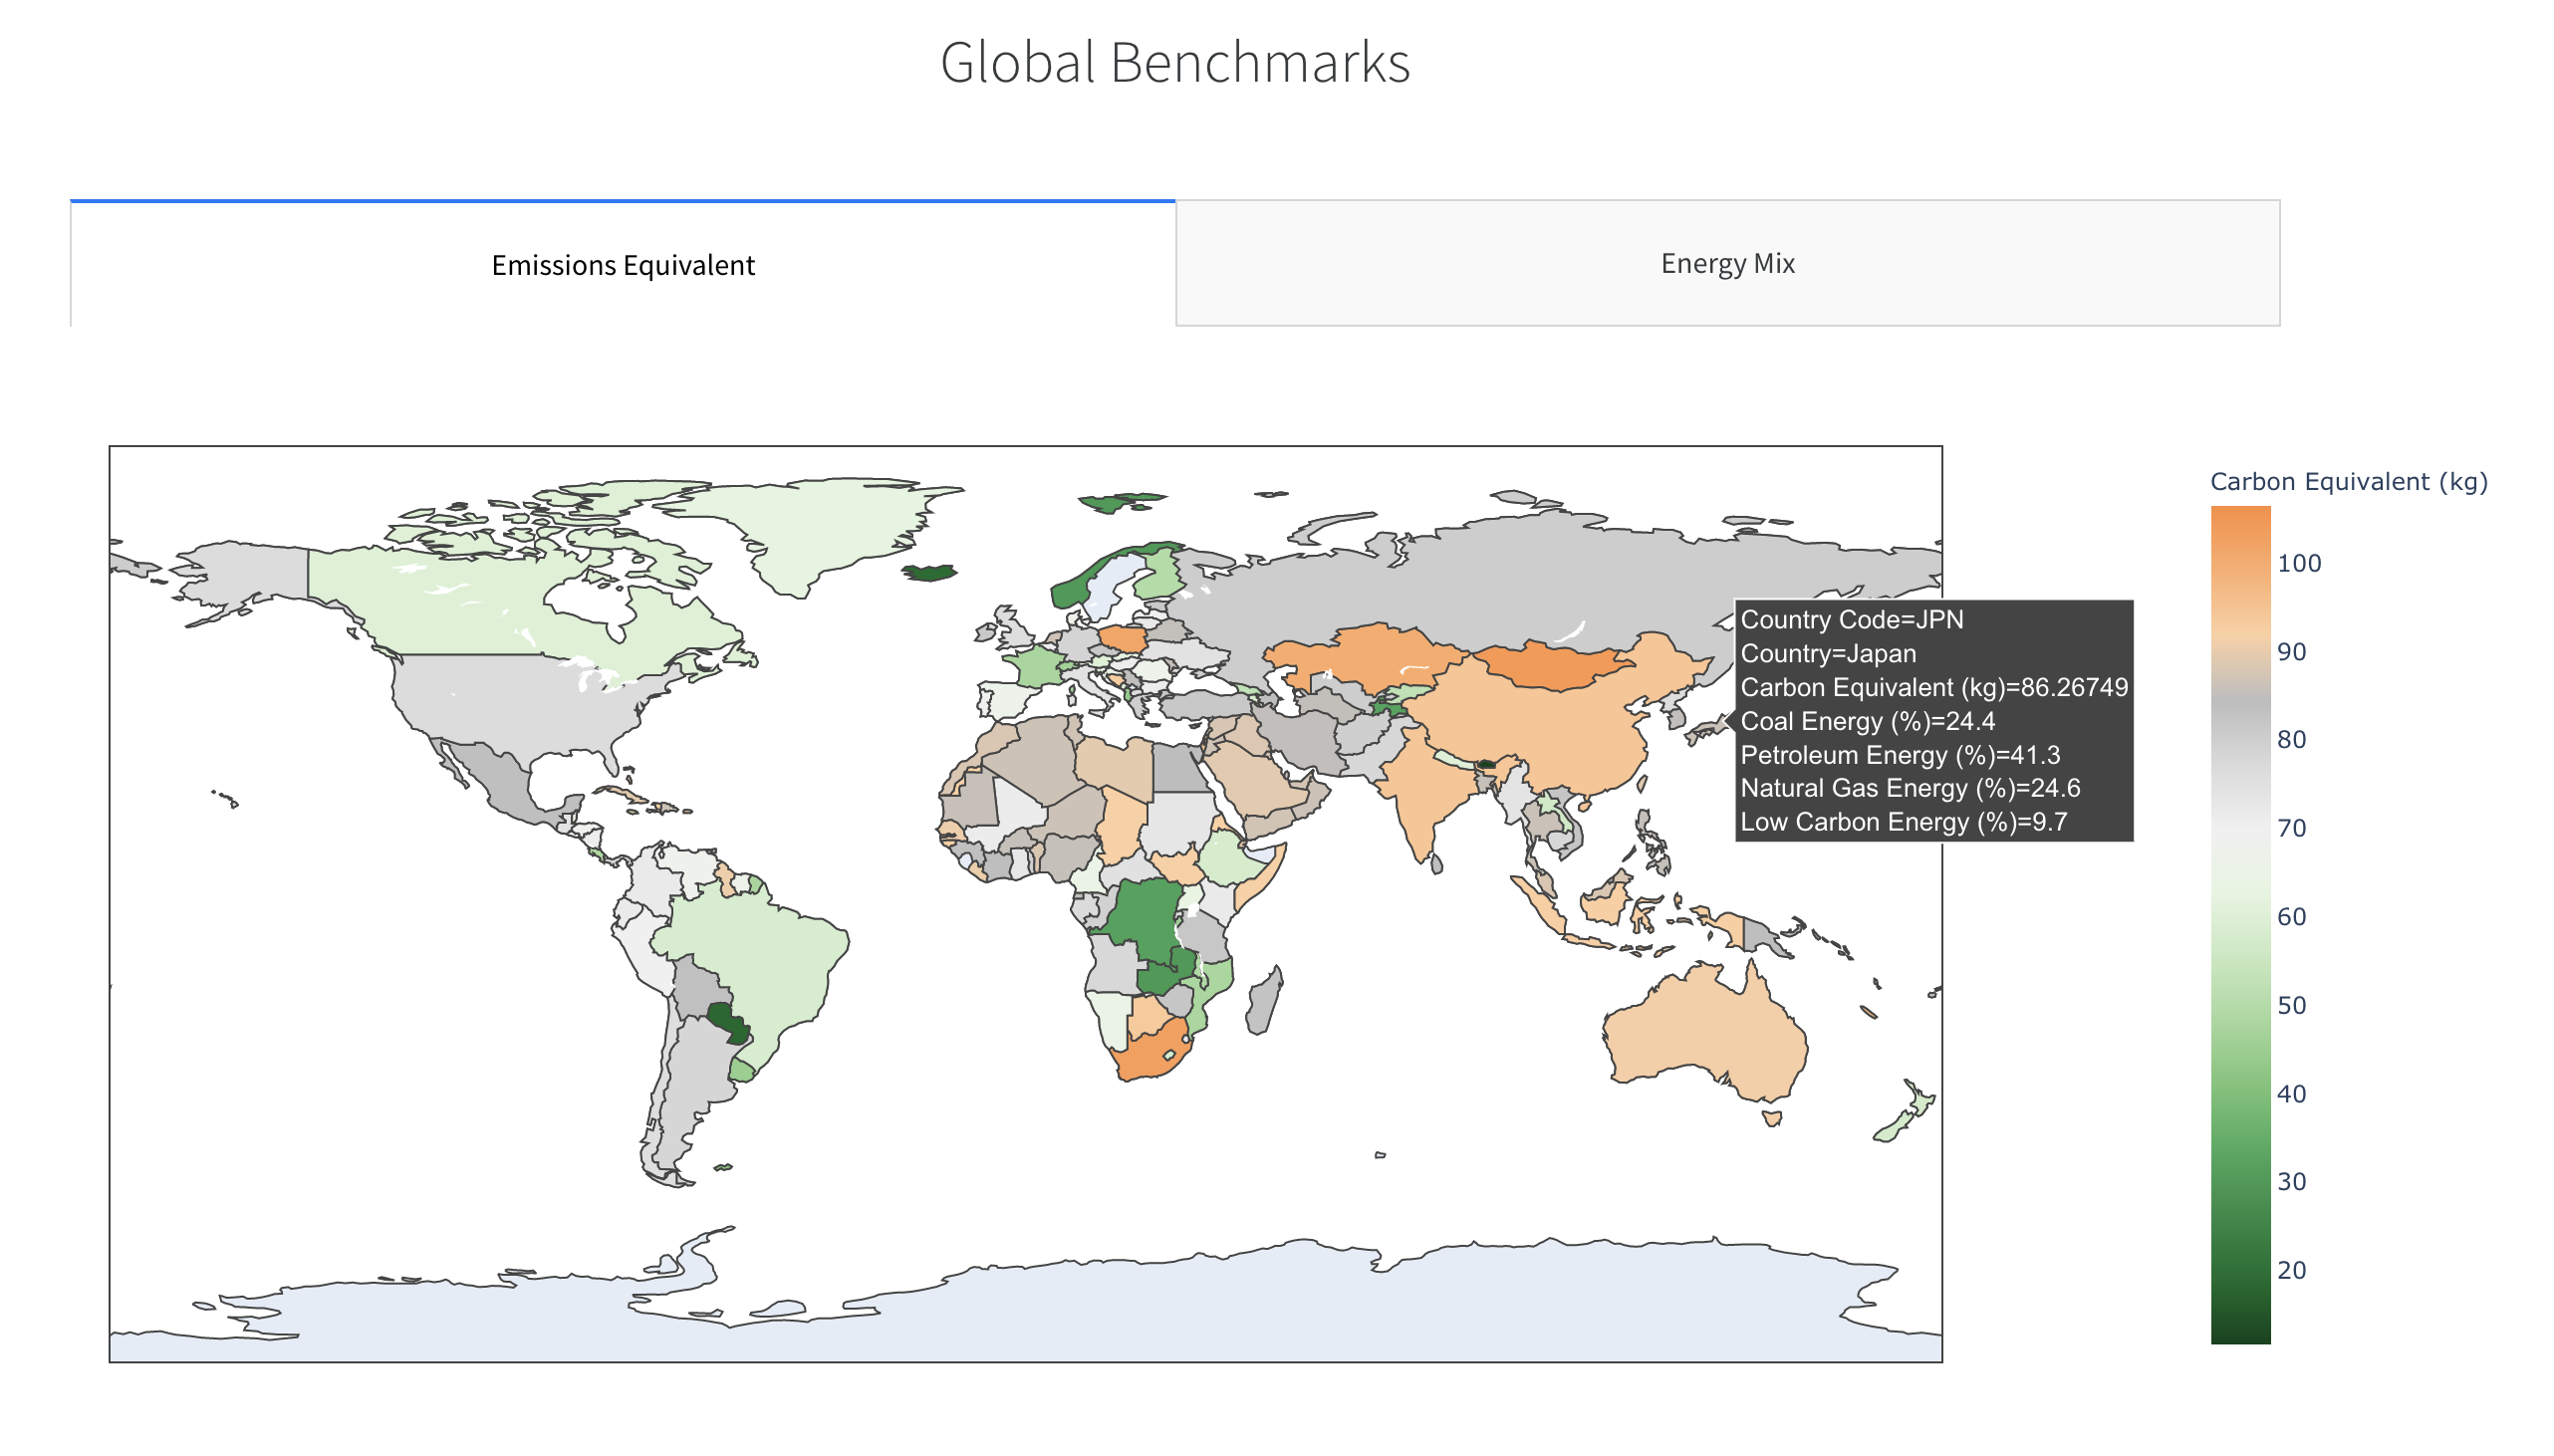
\includegraphics[width=0.9\textwidth]{imagenes/CC_2.png}
\end{center}

\textbf{Online}, si permites subir datos a la API pública de CodeCarbon, accediendo a un dashboard web:

\begin{center}
  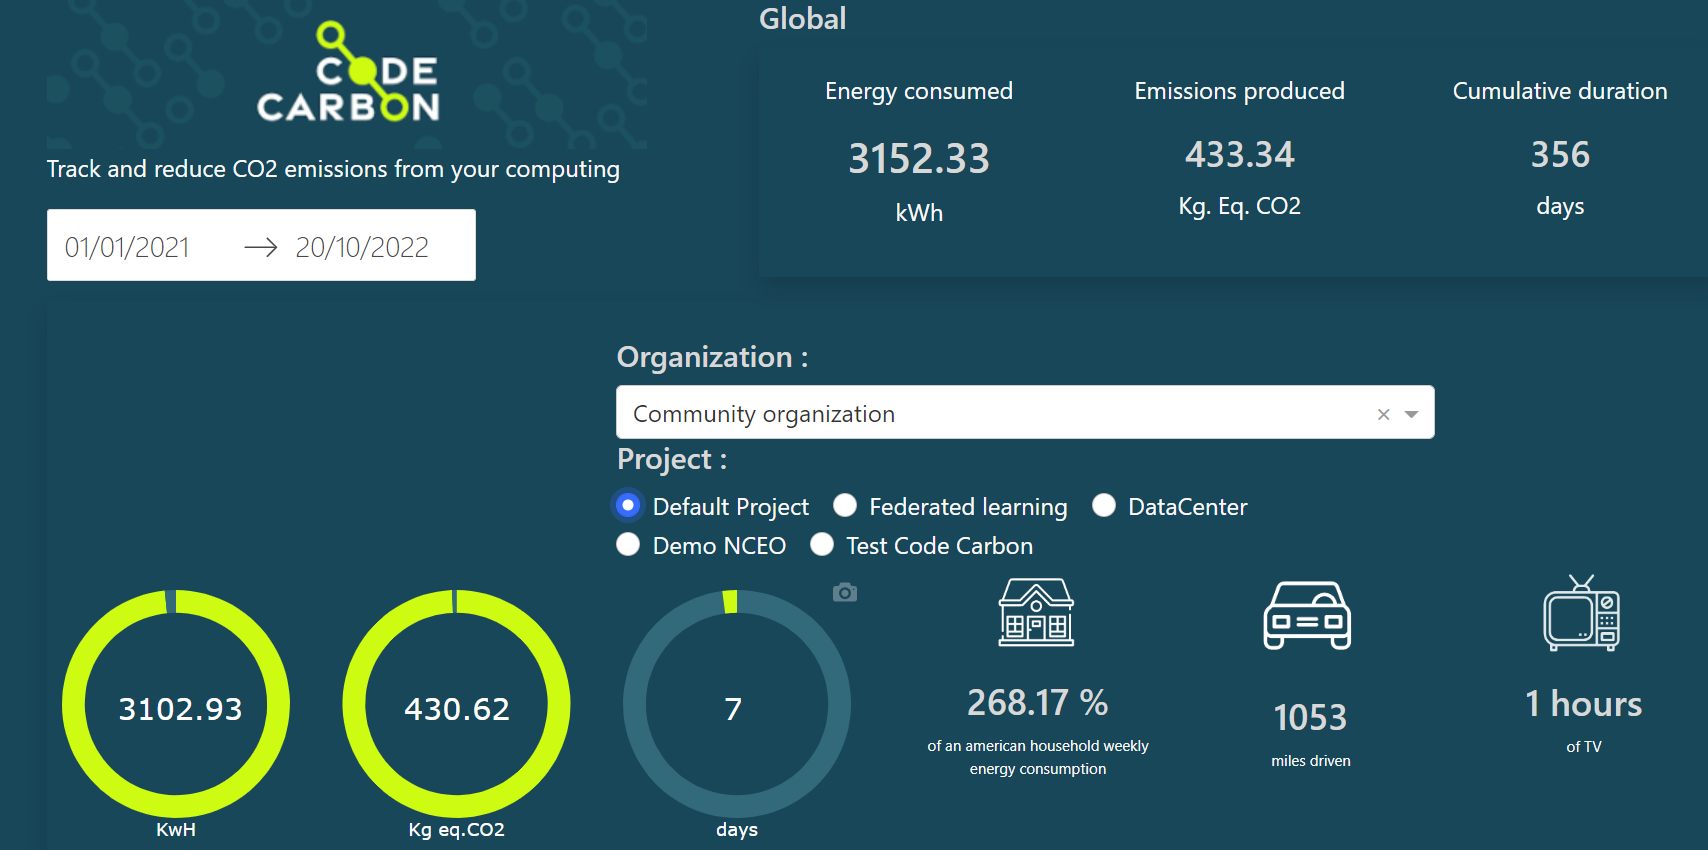
\includegraphics[width=0.9\textwidth]{imagenes/CC_3.png}
\end{center}

\begin{center}
  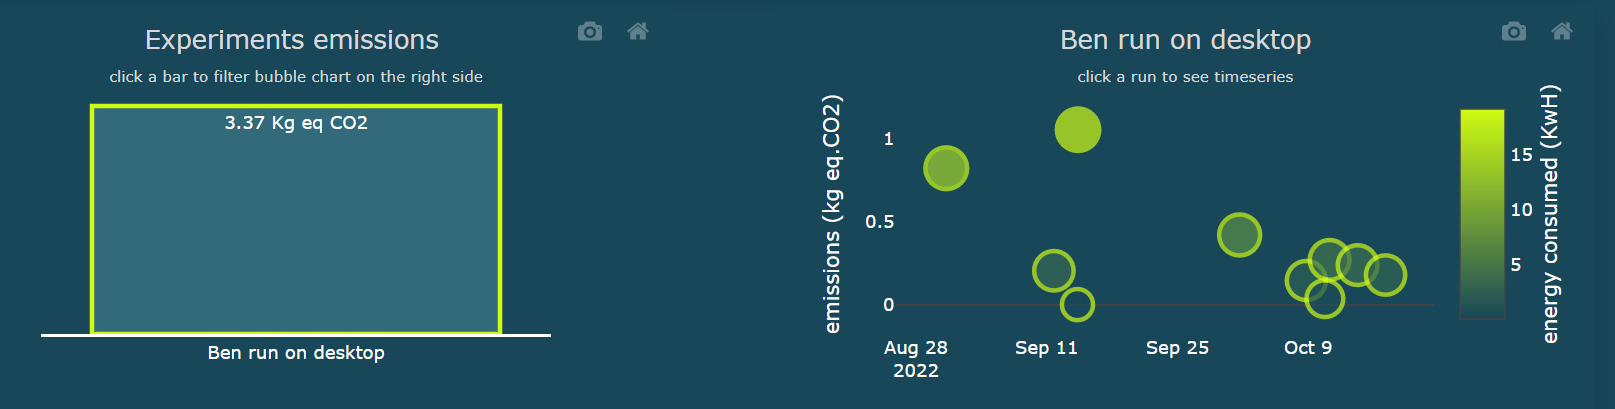
\includegraphics[width=0.9\textwidth]{imagenes/CC_4.png}
\end{center}

\begin{center}
  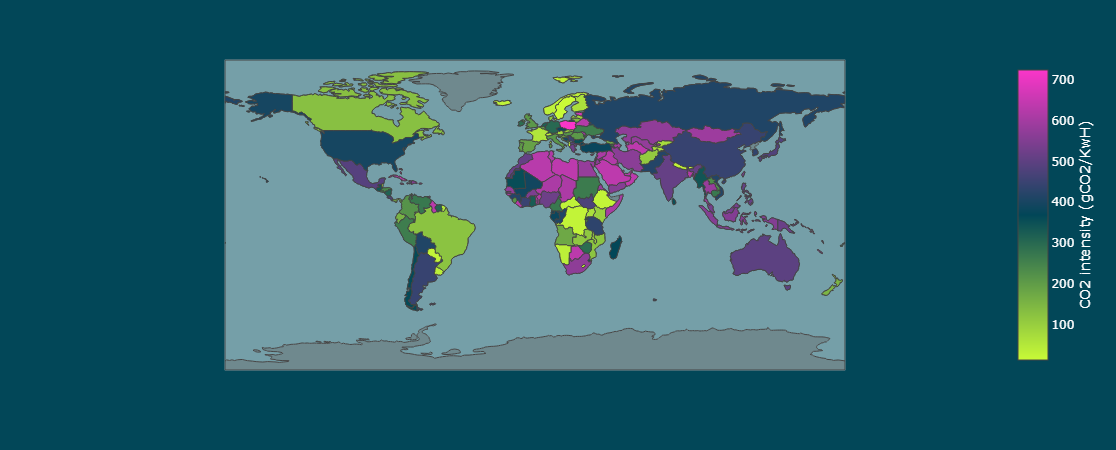
\includegraphics[width=0.9\textwidth]{imagenes/CC_5.png}
\end{center}

\textbf{Puntos fuertes:}
\begin{itemize}
  \item \textbf{Integración sencilla en Python}: basta con añadir un \textbf{decorador\textsuperscript{2}} o usar un bloque \texttt{with}, sin alterar significativamente el código.
  \item \textbf{Contextualización clara de resultados}: incluye equivalencias (km en coche, horas de televisión) para entender el impacto.
  \item \textbf{Modos online y offline}: online obtiene intensidad de carbono actualizada vía APIs como \textbf{ElectricityMap}\footnote{Servicio que ofrece datos sobre intensidad de carbono del consumo eléctrico en tiempo real.}; offline permite especificar región manualmente (códigos ISO).
  \item \textbf{Ligero y eficiente}: pensado para no ralentizar significativamente los procesos.
  \item \textit{Útil en notebooks, scripts y pipelines de \textbf{CI/CD}}: encaja en \textbf{Jupyter Notebooks}\footnote{Entorno interactivo para escribir y ejecutar código en Python.}, *scripts* y cualquier pipeline mediante \textbf{CLI} o decoradores.
  \item \textbf{Comunidad activa y bien documentado}: disponible en \textbf{PyPI\textsuperscript{12}}, con ejemplos y documentación clara.
\end{itemize}

\textbf{Puntos débiles:}
\begin{itemize}
  \item \textbf{Dependencia de datos externos}: precisión limitada si la API de intensidad de carbono no está actualizada.
  \item \textbf{Sin simulaciones de usuario}: no mide flujos de interacción reales, solo bloques de código.
  \item \textbf{Requiere configuración previa}: es necesario generar y gestionar el archivo de configuración.
  \item \textbf{Almacenamiento local}: offline solo guarda en `.csv`, sin historiales automáticos.
  \item \textbf{Sin API propia para análisis masivo}: no permite evaluar múltiples proyectos simultáneamente desde la web.
\end{itemize}

\begin{section}{\textbf{Conclusiones de la comparativa de herramientas}}

% Comandos para ticks y cruces de colores
\newcommand{\tick}{\textcolor{green!60!black}{\ding{51}}}
\newcommand{\cross}{\textcolor{red}{\ding{55}}}

% Tabla 1: AWS CCFT, Impact Framework, Carbon Aware SDK, Cloud Carbon Footprint, Carbonalyser
\begin{landscape}
\begin{table}[H]
\centering
\renewcommand{\arraystretch}{1.3}
\scriptsize
\rowcolors{2}{gray!10}{white}
\begin{tabular}{|p{4.2cm}|c|c|c|c|c|}
\hline
\rowcolor{gray!30}
\textbf{Criterio} & \textbf{AWS CCFT} & \textbf{Impact Framework} & \textbf{Carbon Aware SDK} & \textbf{Cloud Carbon Footprint} & \textbf{Carbonalyser} \\
\hline
Cobertura multicloud                         & \cross & \tick & \tick & \tick & \cross \\
Integración CI/CD                            & \cross & \tick & \tick & \cross & \cross \\
Código abierto                               & \cross & \tick & \tick & \tick & \tick \\
Visualización de resultados                  & \tick  & \cross & \tick & \tick & \tick \\
Requiere conocimientos técnicos altos        & \cross & \tick & \tick & \cross & \cross \\
Estimación basada en datos reales            & \cross & \cross & \tick & \cross & \cross \\
Históricos/Benchmarking                      & \tick  & \cross & \cross & \tick & \cross \\
Personalización/Plugins                      & \cross & \tick & \tick & \cross & \cross \\
Fácil de usar                                & \cross & \cross & \cross & \cross & \tick \\
Análisis detallado (CPU, red, memoria, etc.) & \tick  & \cross & \tick & \tick & \cross \\
% Nuevos criterios
Recomendaciones automáticas                  & \cross & \cross & \cross & \tick & \cross \\
Soporte backend y frontend                   & \cross & \tick & \tick & \tick & \cross \\
Licencia y coste                             & \cross & \tick & \tick & \tick & \tick \\
Actualización y mantenimiento activo         & \tick  & \tick & \tick & \tick & \cross \\
Interfaz de Usuario                          & \tick  & \cross & \cross & \tick & \tick \\
\hline
\end{tabular}
\caption{Comparativa visual de puntos clave (I). \tick: Sí / Ventajoso, \cross: No / Limitado}
\end{table}
\end{landscape}

% Tabla 2: GreenFrame, Website Carbon, Ecograder, CodeCarbon
\begin{landscape}
\begin{table}[H]
\centering
\renewcommand{\arraystretch}{1.3}
\scriptsize
\rowcolors{2}{gray!10}{white}
\begin{tabular}{|p{4.2cm}|c|c|c|c|}
\hline
\rowcolor{gray!30}
\textbf{Criterio} & \textbf{GreenFrame} & \textbf{Website Carbon} & \textbf{Ecograder} & \textbf{CodeCarbon} \\
\hline
Cobertura multicloud                         & \tick & \cross & \cross & \tick \\
Integración CI/CD                            & \tick & \cross & \cross & \tick \\
Código abierto                               & \cross & \tick & \tick & \tick \\
Visualización de resultados                  & \tick & \tick & \tick & \tick \\
Requiere conocimientos técnicos altos        & \tick & \cross & \cross & \tick \\
Estimación basada en datos reales            & \tick & \cross & \cross & \tick \\
Históricos/Benchmarking                      & \cross & \cross & \cross & \tick \\
Personalización/Plugins                      & \cross & \cross & \cross & \cross \\
Fácil de usar                                & \cross & \tick & \tick & \cross \\
Análisis detallado (CPU, red, memoria, etc.) & \tick & \cross & \cross & \tick \\
% Nuevos criterios
Recomendaciones automáticas                  & \tick & \tick & \tick & \cross \\
Soporte backend y frontend                   & \tick & \cross & \cross & \tick \\
Licencia y coste                             & \cross & \tick & \tick & \tick \\
Actualización y mantenimiento activo         & \tick & \tick & \tick & \tick \\
Interfaz de Usuario                          & \tick & \tick & \tick & \cross \\
\hline
\end{tabular}
\caption{Comparativa visual de puntos clave (II). \tick: Sí / Ventajoso, \cross: No / Limitado}
\end{table}
\end{landscape}

\end {section}

\chapter{Propuesta de implementación de EcoCode}

\section{Propuesta de valor}

\section{Diseño de la interfaz de usuario}

\chapter{Diseño Técnico}

\section{Historia de desarrollo}

\section{Diseño de pruebas}

\chapter{Documentación}

\section{Publicacion}

\chapter{Conclusiones y trabajos futuros}

% Bibliografía
\chapter*{Bibliografía}
\addcontentsline{toc}{chapter}{Bibliografía}
\begin{thebibliography}{99}
  \bibitem{ref1}\hypertarget{bib:1}{}\href{https://www.acciona.com/es/cambio-climatico}{https://www.acciona.com/es/cambio-climatico}
  \bibitem{ref2}\hypertarget{bib:2}{}\href{https://www.sostenibilidad.com/cambio-climatico/impactos-cambio-climatico/}{https://www.sostenibilidad.com/cambio-climatico/impactos-cambio-climatico/}
  \bibitem{ref3}\hypertarget{bib:3}{}\href{https://www.who.int/es/news-room/fact-sheets/detail/climate-change-and-health}{https://www.who.int/es/news-room/fact-sheets/detail/climate-change-and-health}
  \bibitem{ref4}\hypertarget{bib:4}{}\href{https://unfccc.int/es/acerca-de-las-ndc/el-acuerdo-de-paris}{https://unfccc.int/es/acerca-de-las-ndc/el-acuerdo-de-paris}
  \bibitem{ref5}\hypertarget{bib:5}{}\href{https://learn.greensoftware.foundation/es/carbon-efficiency/}{https://learn.greensoftware.foundation/es/carbon-efficiency/}
  \bibitem{ref6}\hypertarget{bib:6}{}\href{https://observatorio-ametic.ai/es/inteligencia-artificial-en-sostenibilidad/el-consumo-energetico-de-la-ia-generativa}{https://observatorio-ametic.ai/es/inteligencia-artificial-en-sostenibilidad/el-consumo-energetico-de-la-ia-generativa}
\end{thebibliography}

\end{document}
